\documentclass[a4paper, notitlepage]{report}
\begin{titlepage}

\begin{center}

%% Insert the TU Delft logo at the bottom of the page.
\begin{tikzpicture}[remember picture,overlay]
    \node at (current page.south)[anchor=south,inner sep=0pt]{
        
\includegraphics{cover/logo}
    };
\end{tikzpicture}

%% Extra whitespace at the top.
\vspace*{2\bigskipamount}

%% Print the title in cyan.
{\makeatletter
\titlestyle\color{tudelft-cyan}\Huge\@title
\makeatother}

%% Print the optional subtitle in black.
{\makeatletter
\ifx\@subtitle\undefined\else
    \bigskip
    \titlefont\titleshape\LARGE\@subtitle
\fi
\makeatother}

\bigskip
\bigskip

by
%door

\bigskip
\bigskip

%% Print the name of the author.
{\makeatletter
\titlefont\Large\bfseries\@author
\makeatother}

\vfill

in partial fulfillment of the requirements for the degree of
%in overeenstemming met de vereisten voor het verkrijgen van de graad van

\bigskip
\bigskip

{\bfseries Master of Science}

in Applied Physics

\bigskip
\bigskip

at the Delft University of Technology,
%aan de Technische Universiteit Delft,

to be defended publicly on Tuesday January 1, 2013 at 10:00 AM.
%in het openbaar de verdedigen op dinsdag 1 januari om 10:00 uur.

\vfill

\begin{tabular}{lll}
%% Add additional information here, per faculty requirements, e.g
%    Student number: & 1234567 \\
%    Project duration: & \multicolumn{2}{l}{March 1, 2012 -- January 1, 2013} \\
    Supervisor: & Prof.\ dr.\ ir.\ A.\ Einstein \\
    Thesis committee:
        & Prof.\ dr.\ C.\ F.\ Xavier, & TU Delft \\
        & Dr.\ E.\ L.\ Brown, & TU Delft \\
        & Ir.\ M.\ Scott, & Acme Corporation
\end{tabular}

%% Only include the following lines if confidentiality is applicable.
\bigskip
\bigskip
\emph{This thesis is confidential and cannot be made public until December 31, 2013.}
%\emph{Op dit verslag is geheimhouding van toepassing tot en met 31 december 2013.}

\bigskip
\bigskip
An electronic version of this thesis is available at \url{http://repository.tudelft.nl/}.
%Een elektronische versie van dit verslag is beschikbaar op \url{http://repository.tudelft.nl/}.

\end{center}

\end{titlepage}


% All imports needed for file

% General
\usepackage[a4paper,top=1.25in,right=1in,bottom=1.25in,left=1in]{geometry}
\usepackage[utf8]{inputenc}
\usepackage[T1]{fontenc}
\usepackage{textcomp}
\usepackage[bitstream-charter]{mathdesign}
\usepackage{cite}

\usepackage{import}
\usepackage{standalone}
\usepackage{epstopdf}



% Math
\usepackage{amsmath}	% some standard math functions
%\usepackage{amssymb}	% more mathematical symbols
\usepackage{amsbsy}	% enable bold mathematics
\usepackage{bm}
%\usepackage{amsthm}	% enable theorem statements
\usepackage{trfsigns} 	% symbols for transforms

% Text formatting
\usepackage{fancyhdr}	% allow more control over page headers/footers
\usepackage{enumitem}	% allow control over enumerate, itemize, description
\usepackage{setspace}	% allow control over spacing
\usepackage{lastpage}	% provide label for last page in document
\usepackage{sectsty}	% allow control over section styling
\usepackage{url}

% Floats
\usepackage{xcolor}		% enable use of colors
\usepackage{graphicx}		% enable graphics
\usepackage{float}		% enable floats
\usepackage[section]{placeins}	% prevent floats from moving past e.g. sections
\usepackage[small, bf, hang, figurename=Fig.]{caption}	% enable captions for floats (images etc.)
\captionsetup{width=.8\textwidth} % captions not too wide
\usepackage{subcaption}		% enable subcaptions for floats (images etc.)
\usepackage[nottoc]{tocbibind}		% put more stuff in TOC

% Styling data
\pagestyle{fancyplain}

% Title page
\makeatletter
\let\inserttitle\@title
\makeatother

% Page header
\setlength{\headwidth}{\textwidth}
\lhead{} % leave left header empty
\chead{}
\rhead{} % leave right header empty
\lfoot{} % leave left footer empty
\cfoot{} % leave center footer empty
\rfoot{}
\renewcommand{\headrulewidth}{0.3pt}
\renewcommand{\footrulewidth}{0pt}

% Section, equation and figure numbering
\usepackage{chngcntr} 
\counterwithout{figure}{chapter}
\renewcommand{\thechapter}{\Roman{chapter}}
\renewcommand{\thesection}{\Roman{chapter}.\arabic{section}}
\renewcommand{\thesubsection}{\Roman{chapter}.\arabic{section}.\arabic{subsection}}
\renewcommand{\thesubsubsection}{\alph{subsubsection})}
\renewcommand{\thefigure}{\arabic{figure}}
\renewcommand{\thesubfigure}{\alph{subfigure}}
\renewcommand{\theequation}{\thechapter--\arabic{equation}}
\setcounter{tocdepth}{1}
\captionsetup[figure]{labelsep=period}

% Nice enumerations
\newlist{enum}{enumerate}{1}
\setlist[enum]{label=\textbf{[\arabic*]}} % \arabic or \alpha
\setlist{itemsep=-5pt}

% Nice \begin{StateDescription} for FSM descriptions
\newlist{StateDescription}{description}{1}
\setlist[StateDescription]{font=\normalfont\scshape, labelwidth=12em, leftmargin=12em,listparindent=0em,itemindent=0em}

% Section formatting
\definecolor{title-gray}{gray}{0.45}		% grijstint voor headers
\renewcommand*\sfdefault{lmss}
\allsectionsfont{\sffamily\color{title-gray}}	% sans-serif in headers

% Page layout
\onehalfspacing					% Wide margins for text
\usepackage{chngpage}			% customize margins of certain pages
\usepackage{adjustbox}

% Text macros
\usepackage{xspace}
\newcommand{\matlab}{MATLAB\xspace}		% fancy MATLAB command
\newcommand{\norm}[1]{\left\lVert#1\right\rVert}% Command for vector norm
\newcommand{\abs}[1]{\left\lvert#1\right\rvert}% Command for abs
\newcommand{\todo}[1]{\textbf{\textcolor{red}{#1}}}	% placeholder stuff
\let\oldhat\hat
\renewcommand{\vec}[1]{\bm{#1}} % bold vectors in math mode
\newcommand{\vechat}[1]{\oldhat{\bm{#1}}} % hat in vector mode
\newcommand{\mat}[1]{\bm{#1}} % bold matrix in math mode

%links
\usepackage{hyperref}
\hypersetup{ %setup hyperlinks
    colorlinks=true,
    citecolor=black,
    filecolor=black,
    linkcolor=black,
    urlcolor=black
}


\begin{document}
\lhead{\fancyplain{}{\textsf{\nouppercase{\leftmark}}}} % Appendix in header

\appendix
\renewcommand{\thechapter}{\Alph{chapter}}
\renewcommand{\thesection}{\Roman{section}}
\chapter{Full simulation and experiment results}
\label{app:results}
\vspace{-35pt}
\section{Orientation measurements}
\begin{figure}[H]
\begin{adjustwidth}{-1in}{-1in}
\centering
	\begin{subfigure}{0.33\textwidth}
		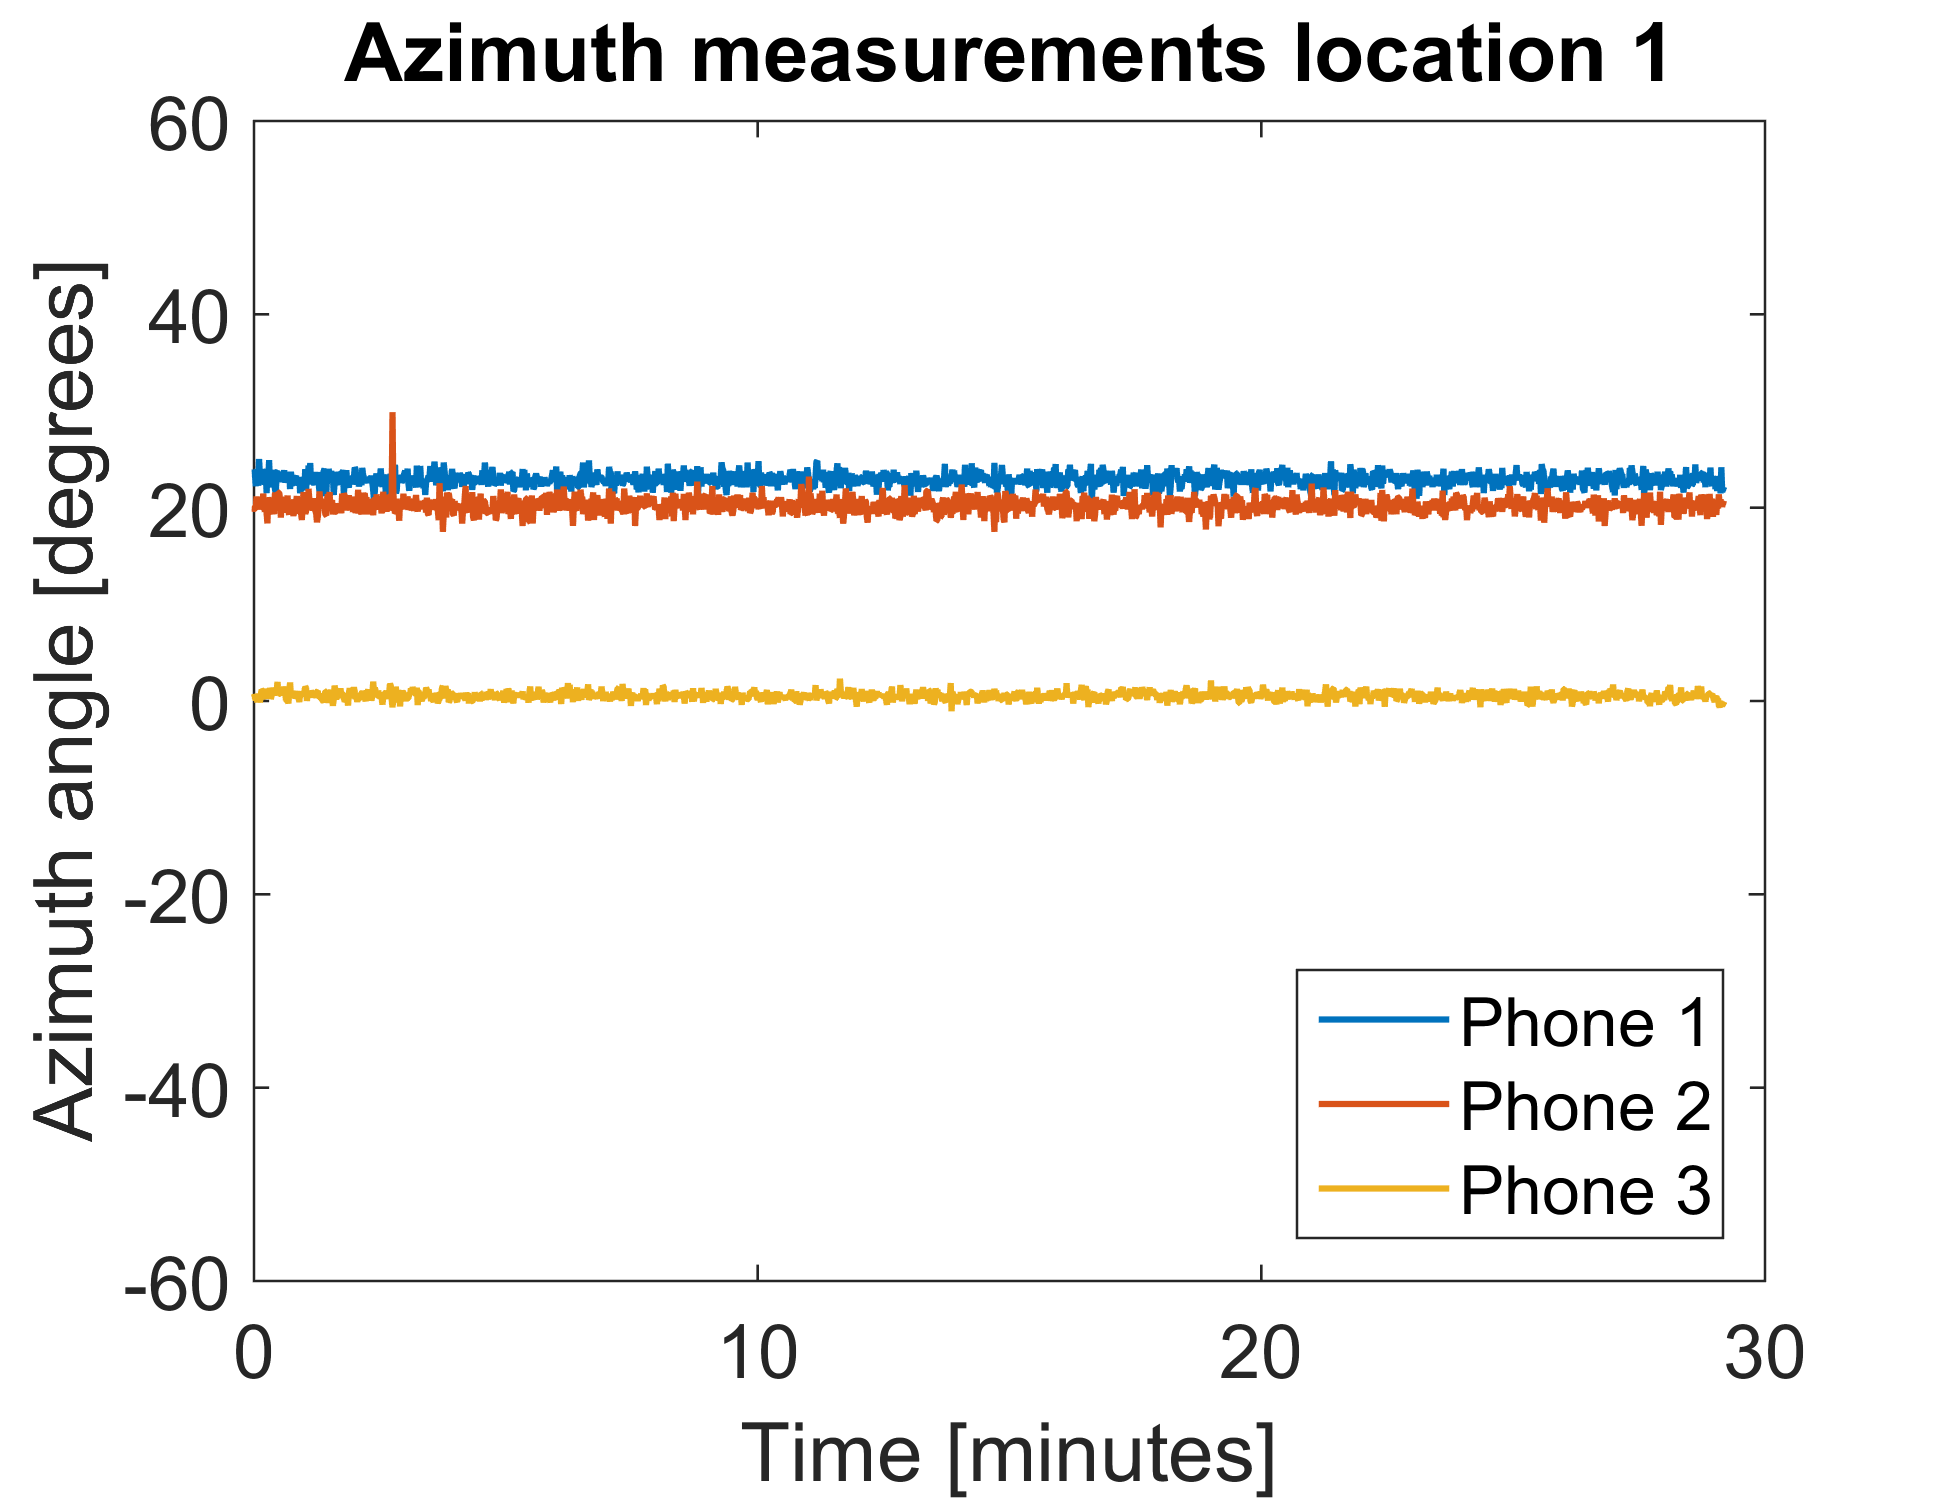
\includegraphics[width=\textwidth]{figures/orientation/az_loc1}
		\caption{Azimuth angles for location 1.}
		\label{app:orientation_az_loc1}
	\end{subfigure}
	\begin{subfigure}{0.33\textwidth}
		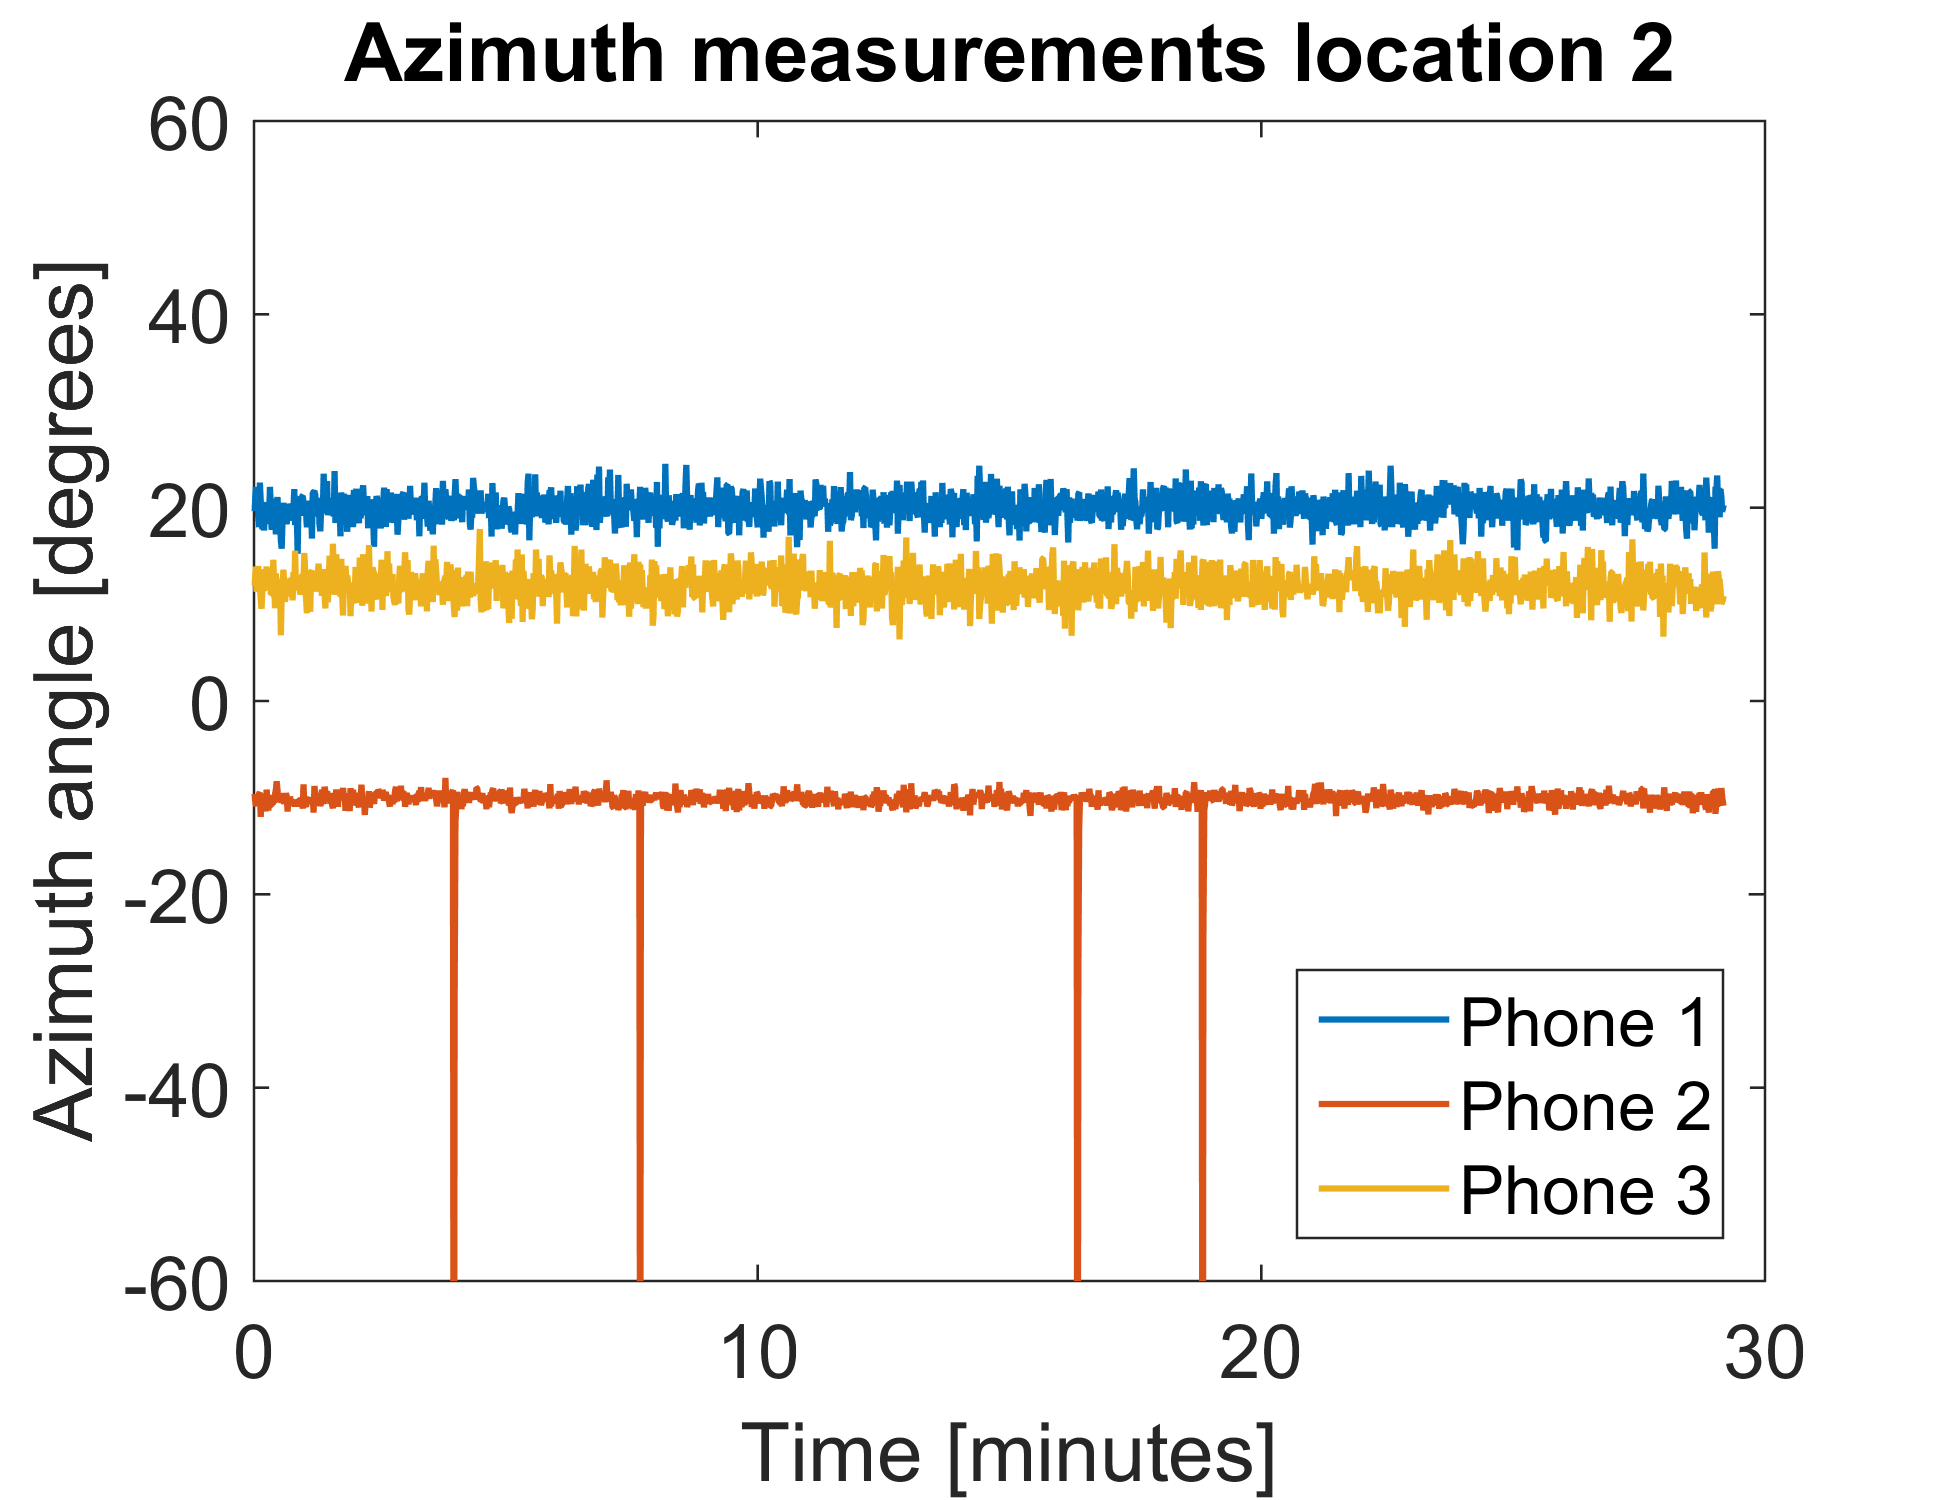
\includegraphics[width=\textwidth]{figures/orientation/az_loc2}
		\caption{Azimuth angles for location 2.}
		\label{app:orientation_az_loc2}
	\end{subfigure}
	\begin{subfigure}{0.33\textwidth}
		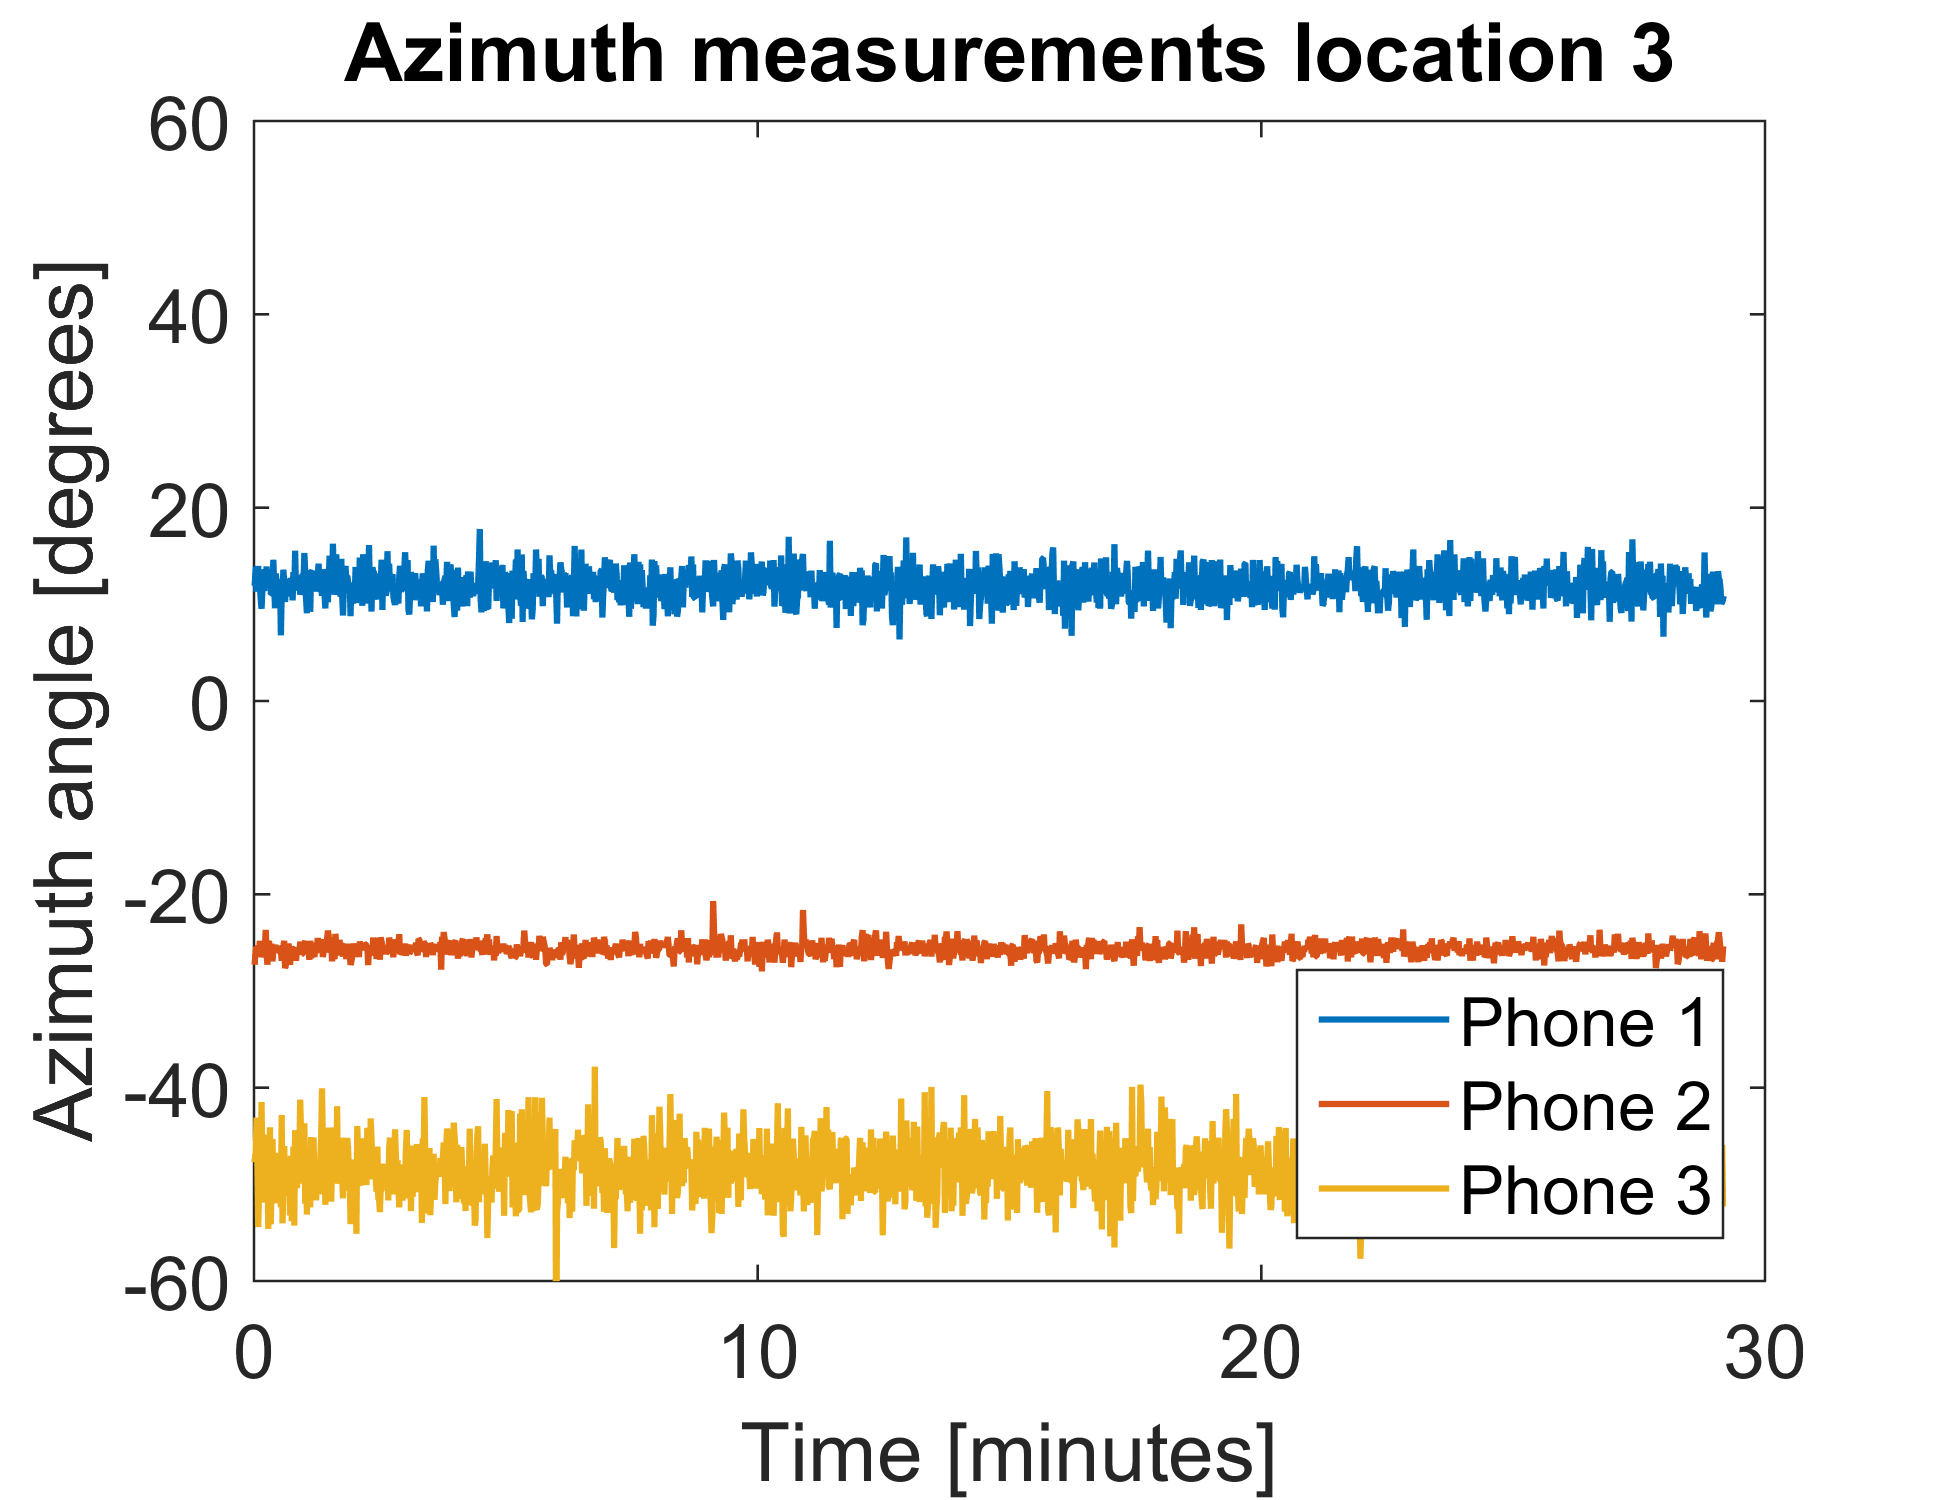
\includegraphics[width=\textwidth]{figures/orientation/az_loc3}
		\caption{Azimuth angles for location 3.}
		\label{app:orientation_az_loc3}
	\end{subfigure}
	
	\vspace{10pt}
	\begin{subfigure}{0.33\textwidth}
		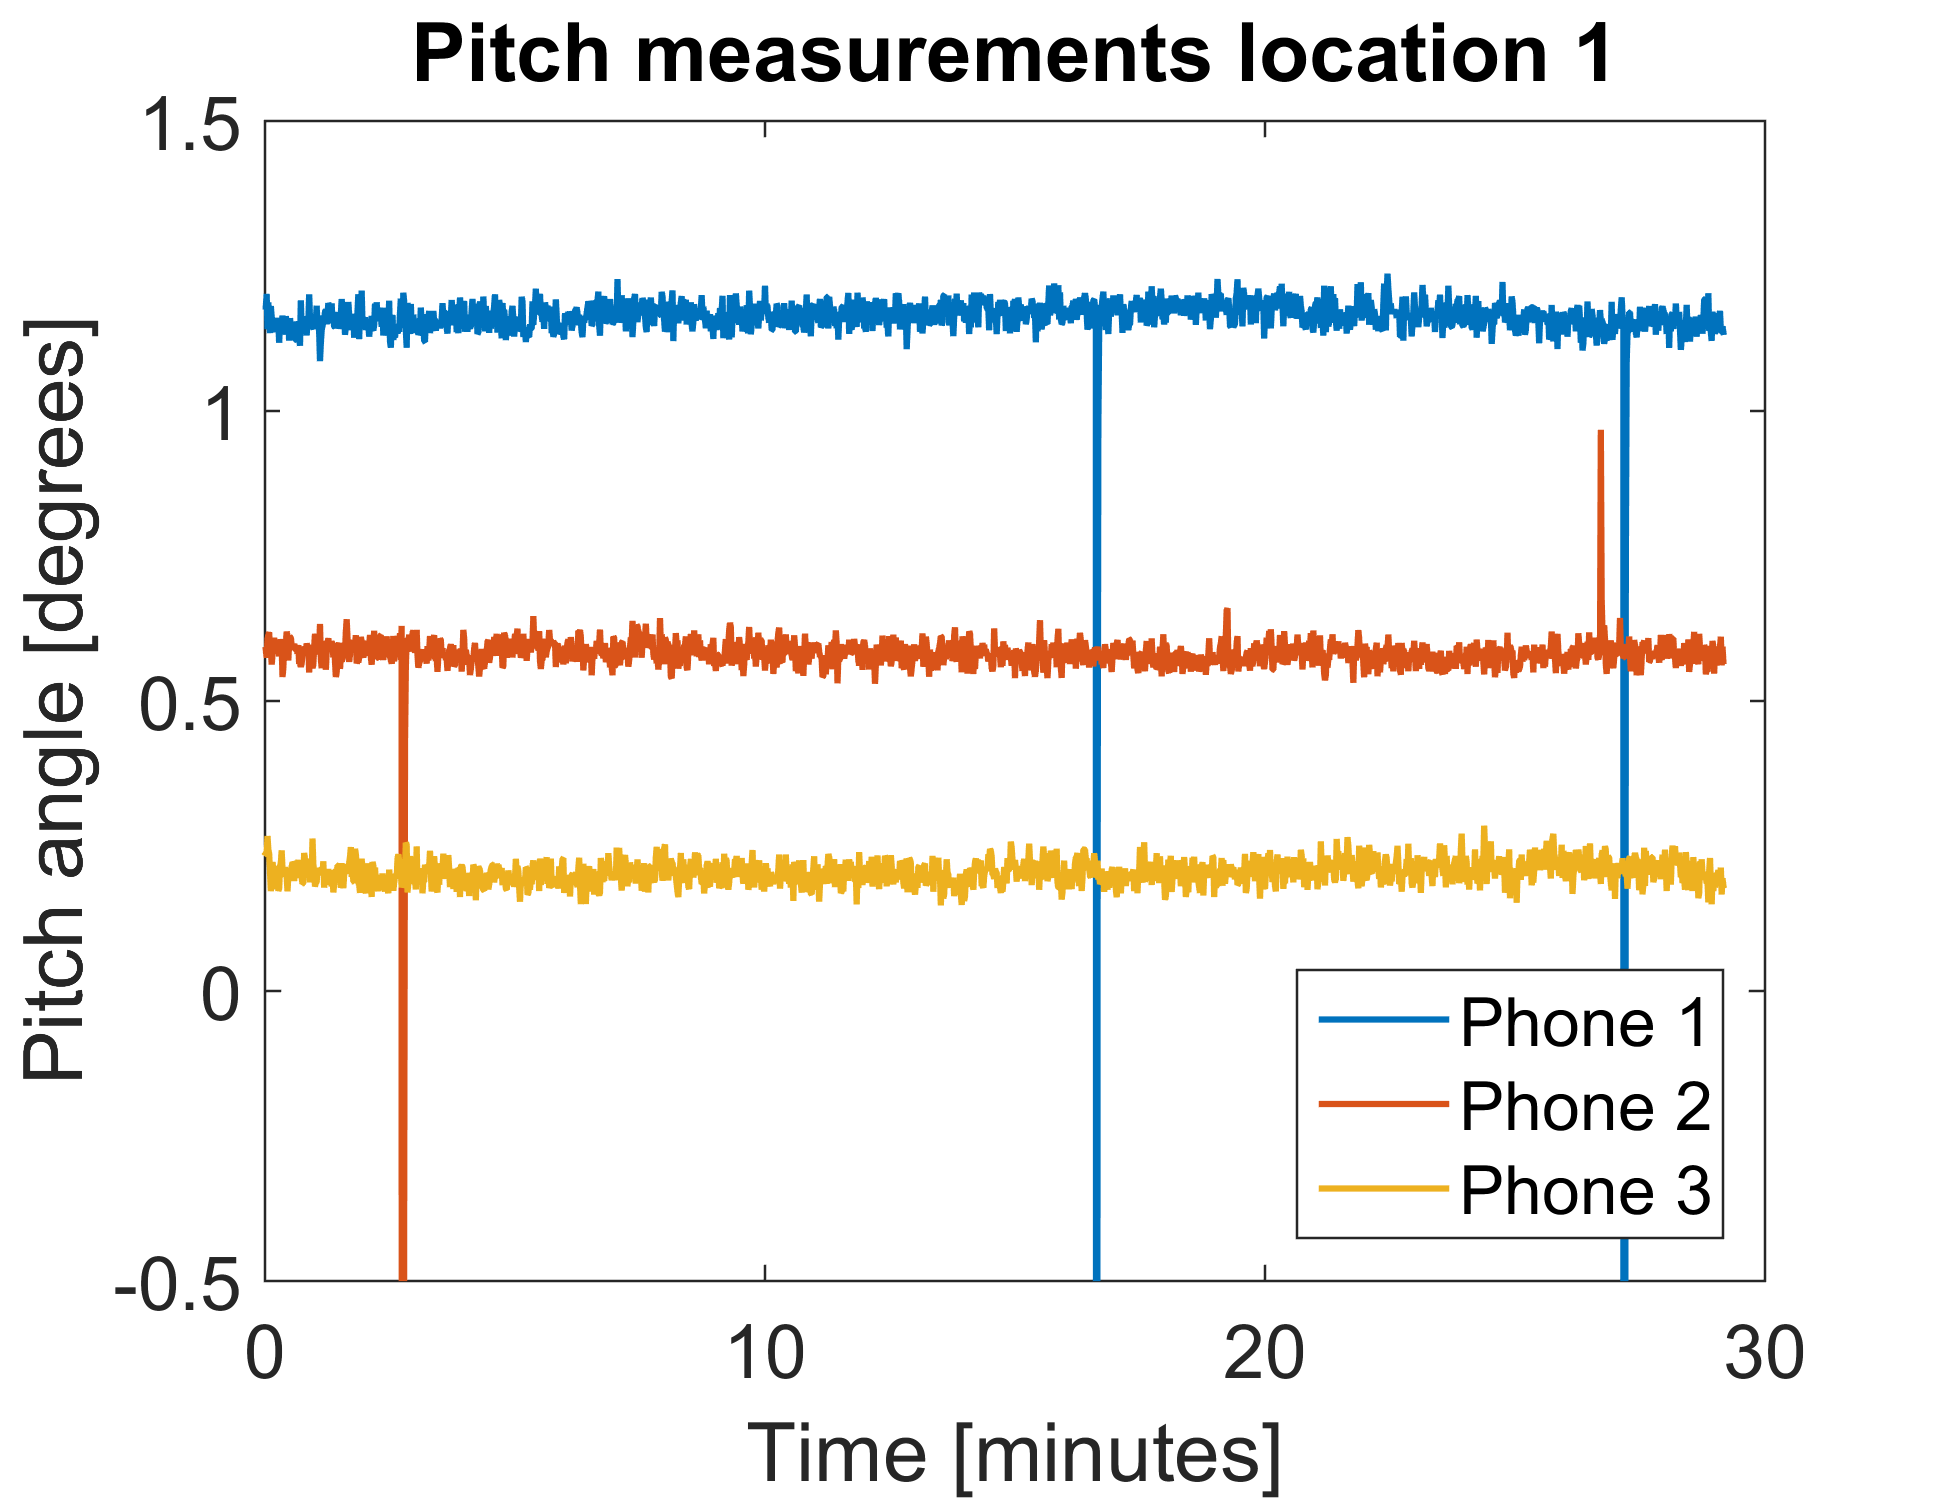
\includegraphics[width=\textwidth]{figures/orientation/pi_loc1}
		\caption{Pitch angles for location 1.}
		\label{app:orientation_pi_loc1}
	\end{subfigure}
	\begin{subfigure}{0.33\textwidth}
		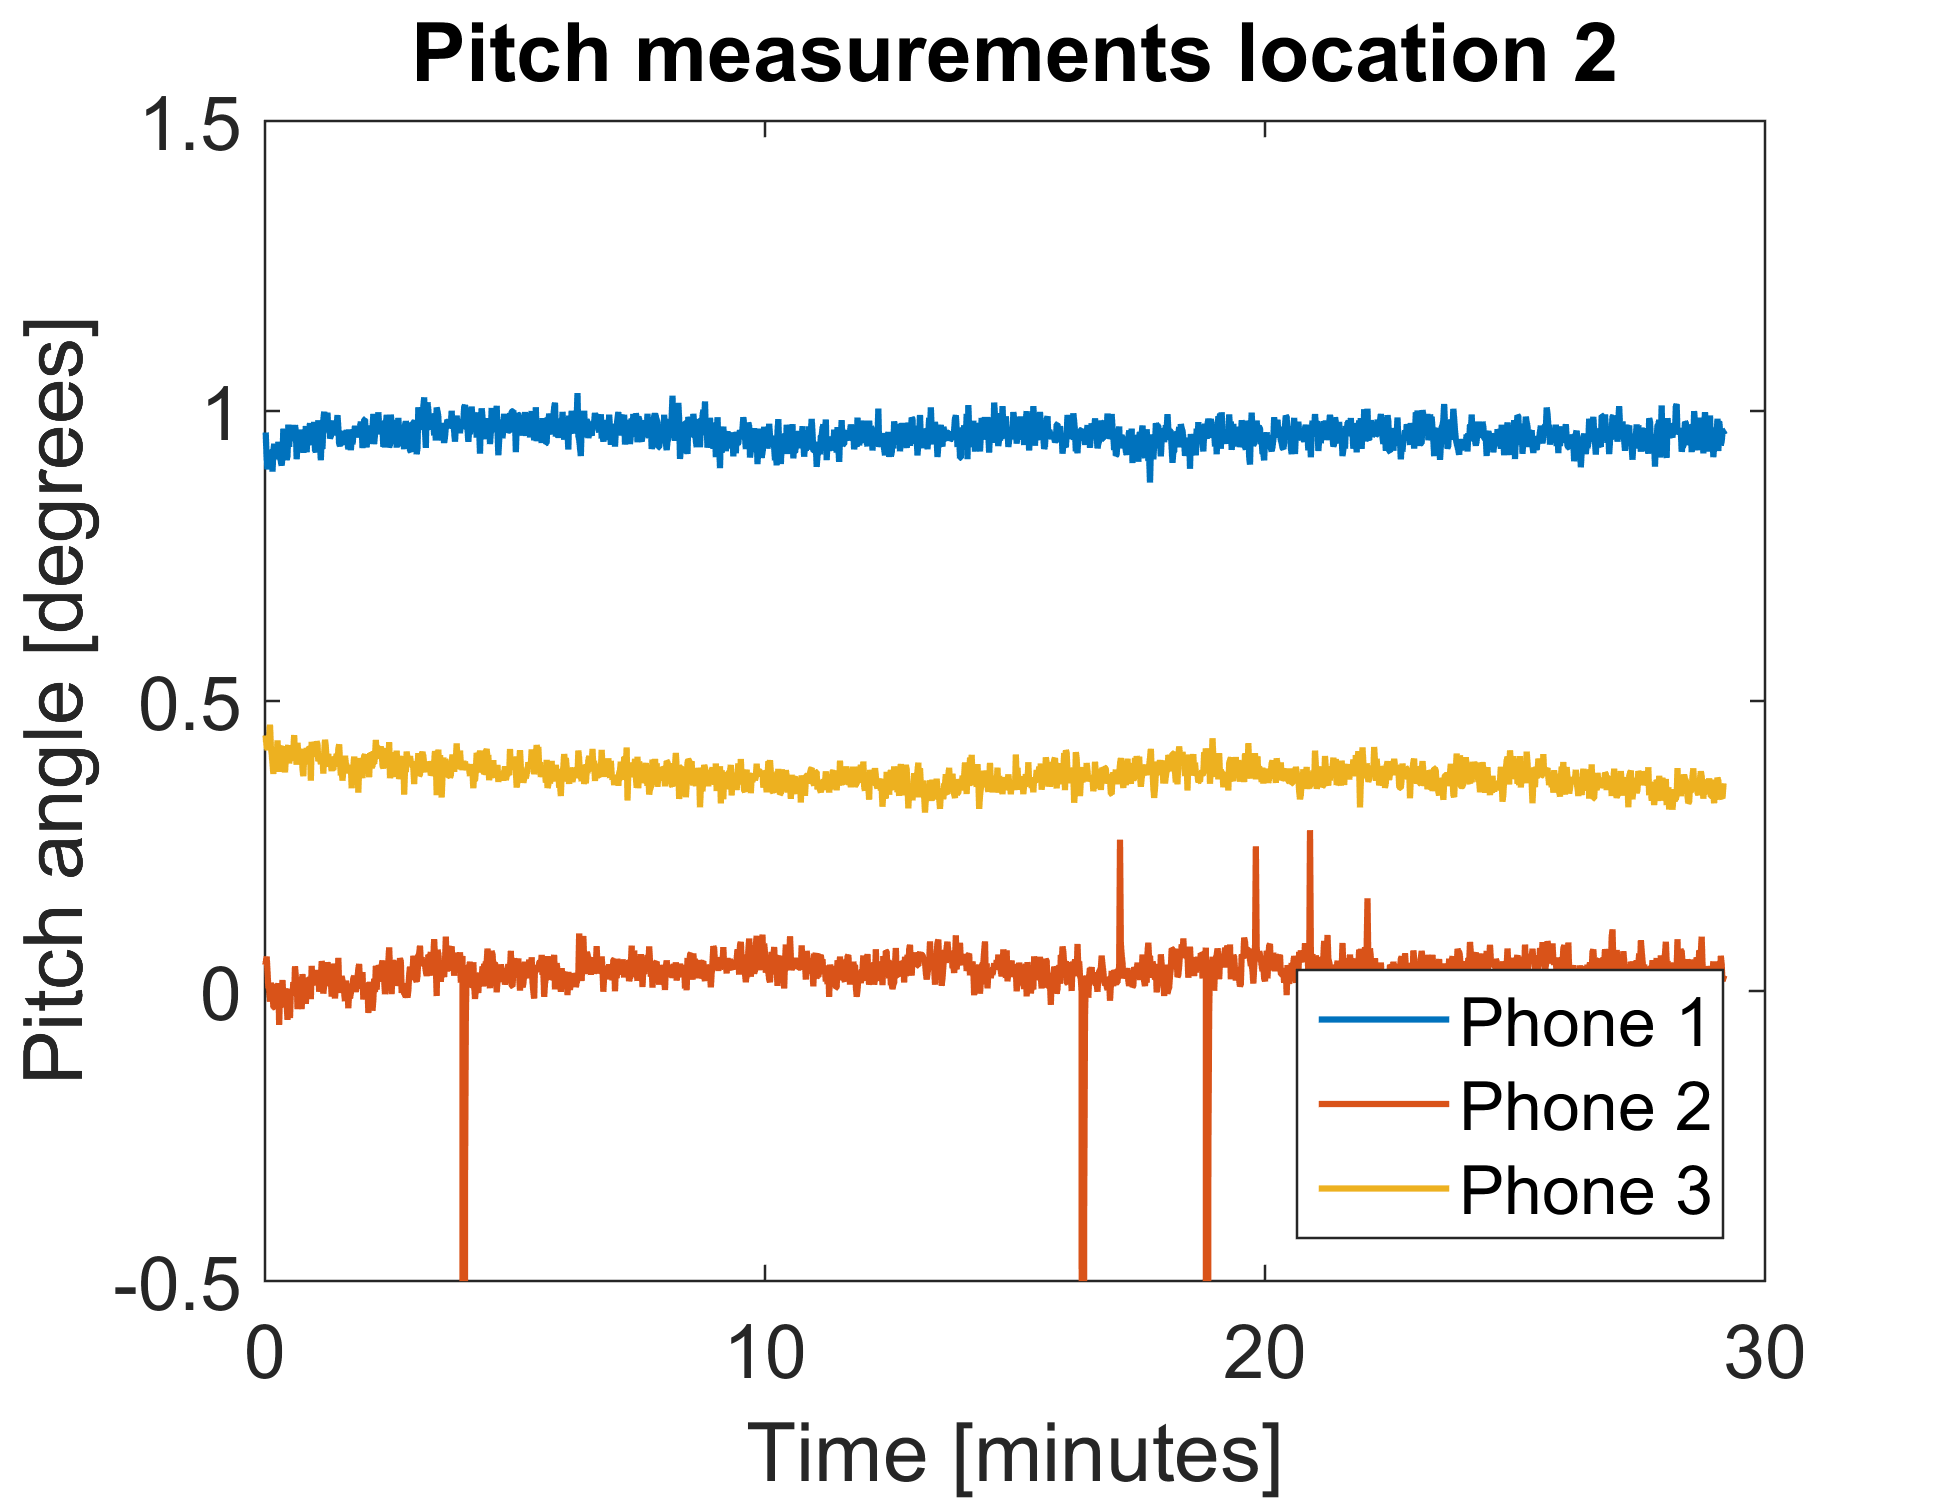
\includegraphics[width=\textwidth]{figures/orientation/pi_loc2}
		\caption{Pitch angles for location 2.}
		\label{app:orientation_pi_loc2}
	\end{subfigure}
	\begin{subfigure}{0.33\textwidth}
		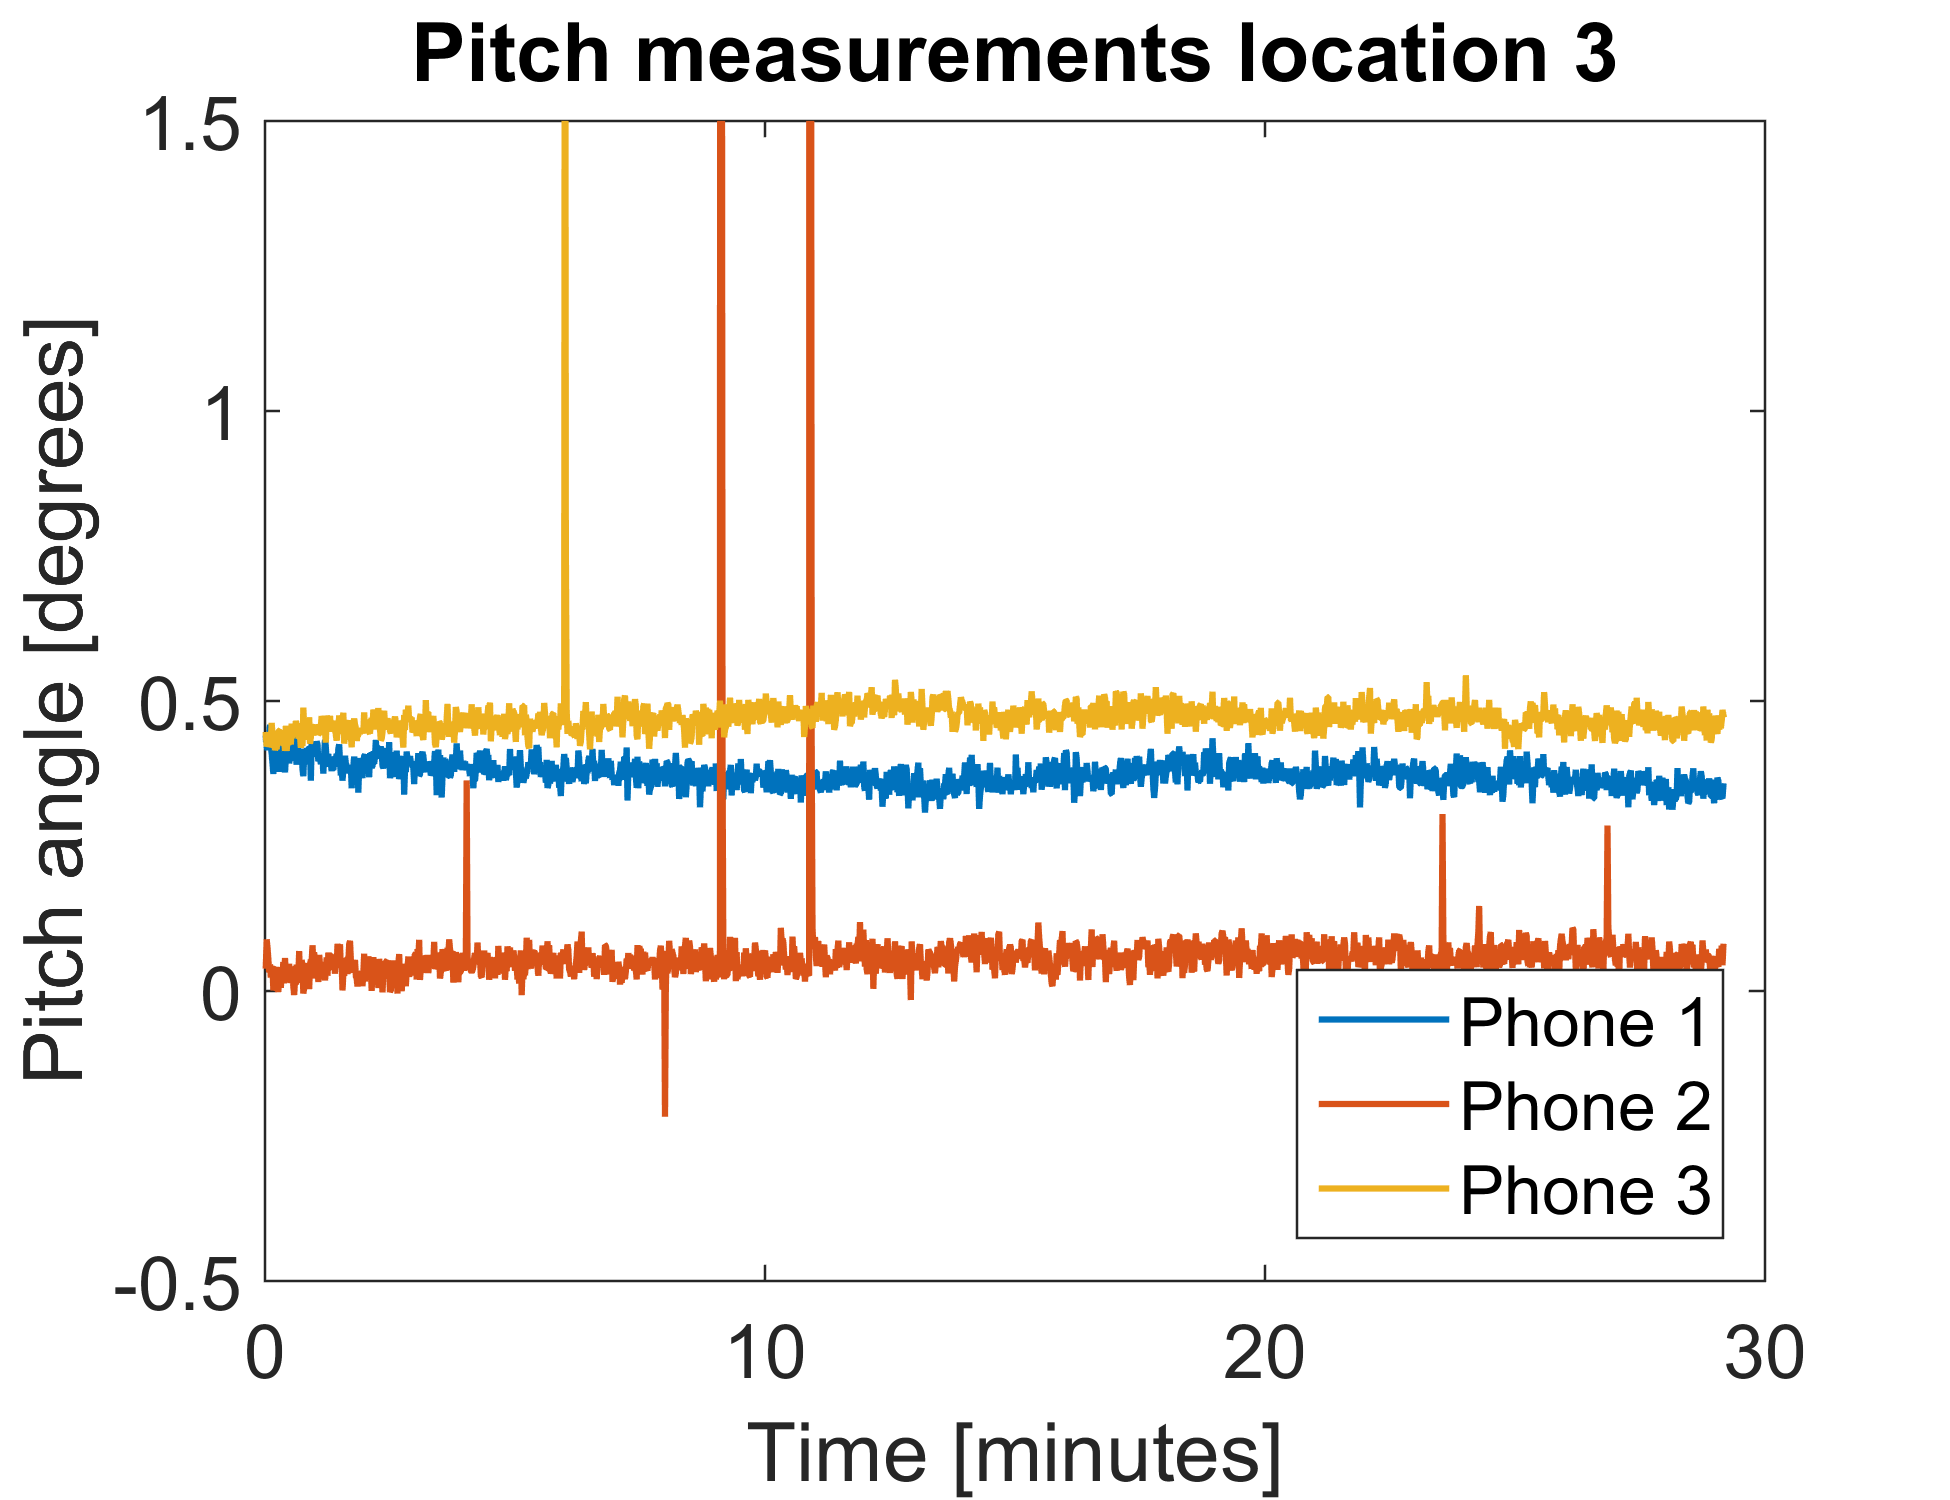
\includegraphics[width=\textwidth]{figures/orientation/pi_loc3}
		\caption{Pitch angles for location 3.}
		\label{app:orientation_pi_loc3}
	\end{subfigure}	
	
	\vspace{10pt}
	\begin{subfigure}{0.33\textwidth}
		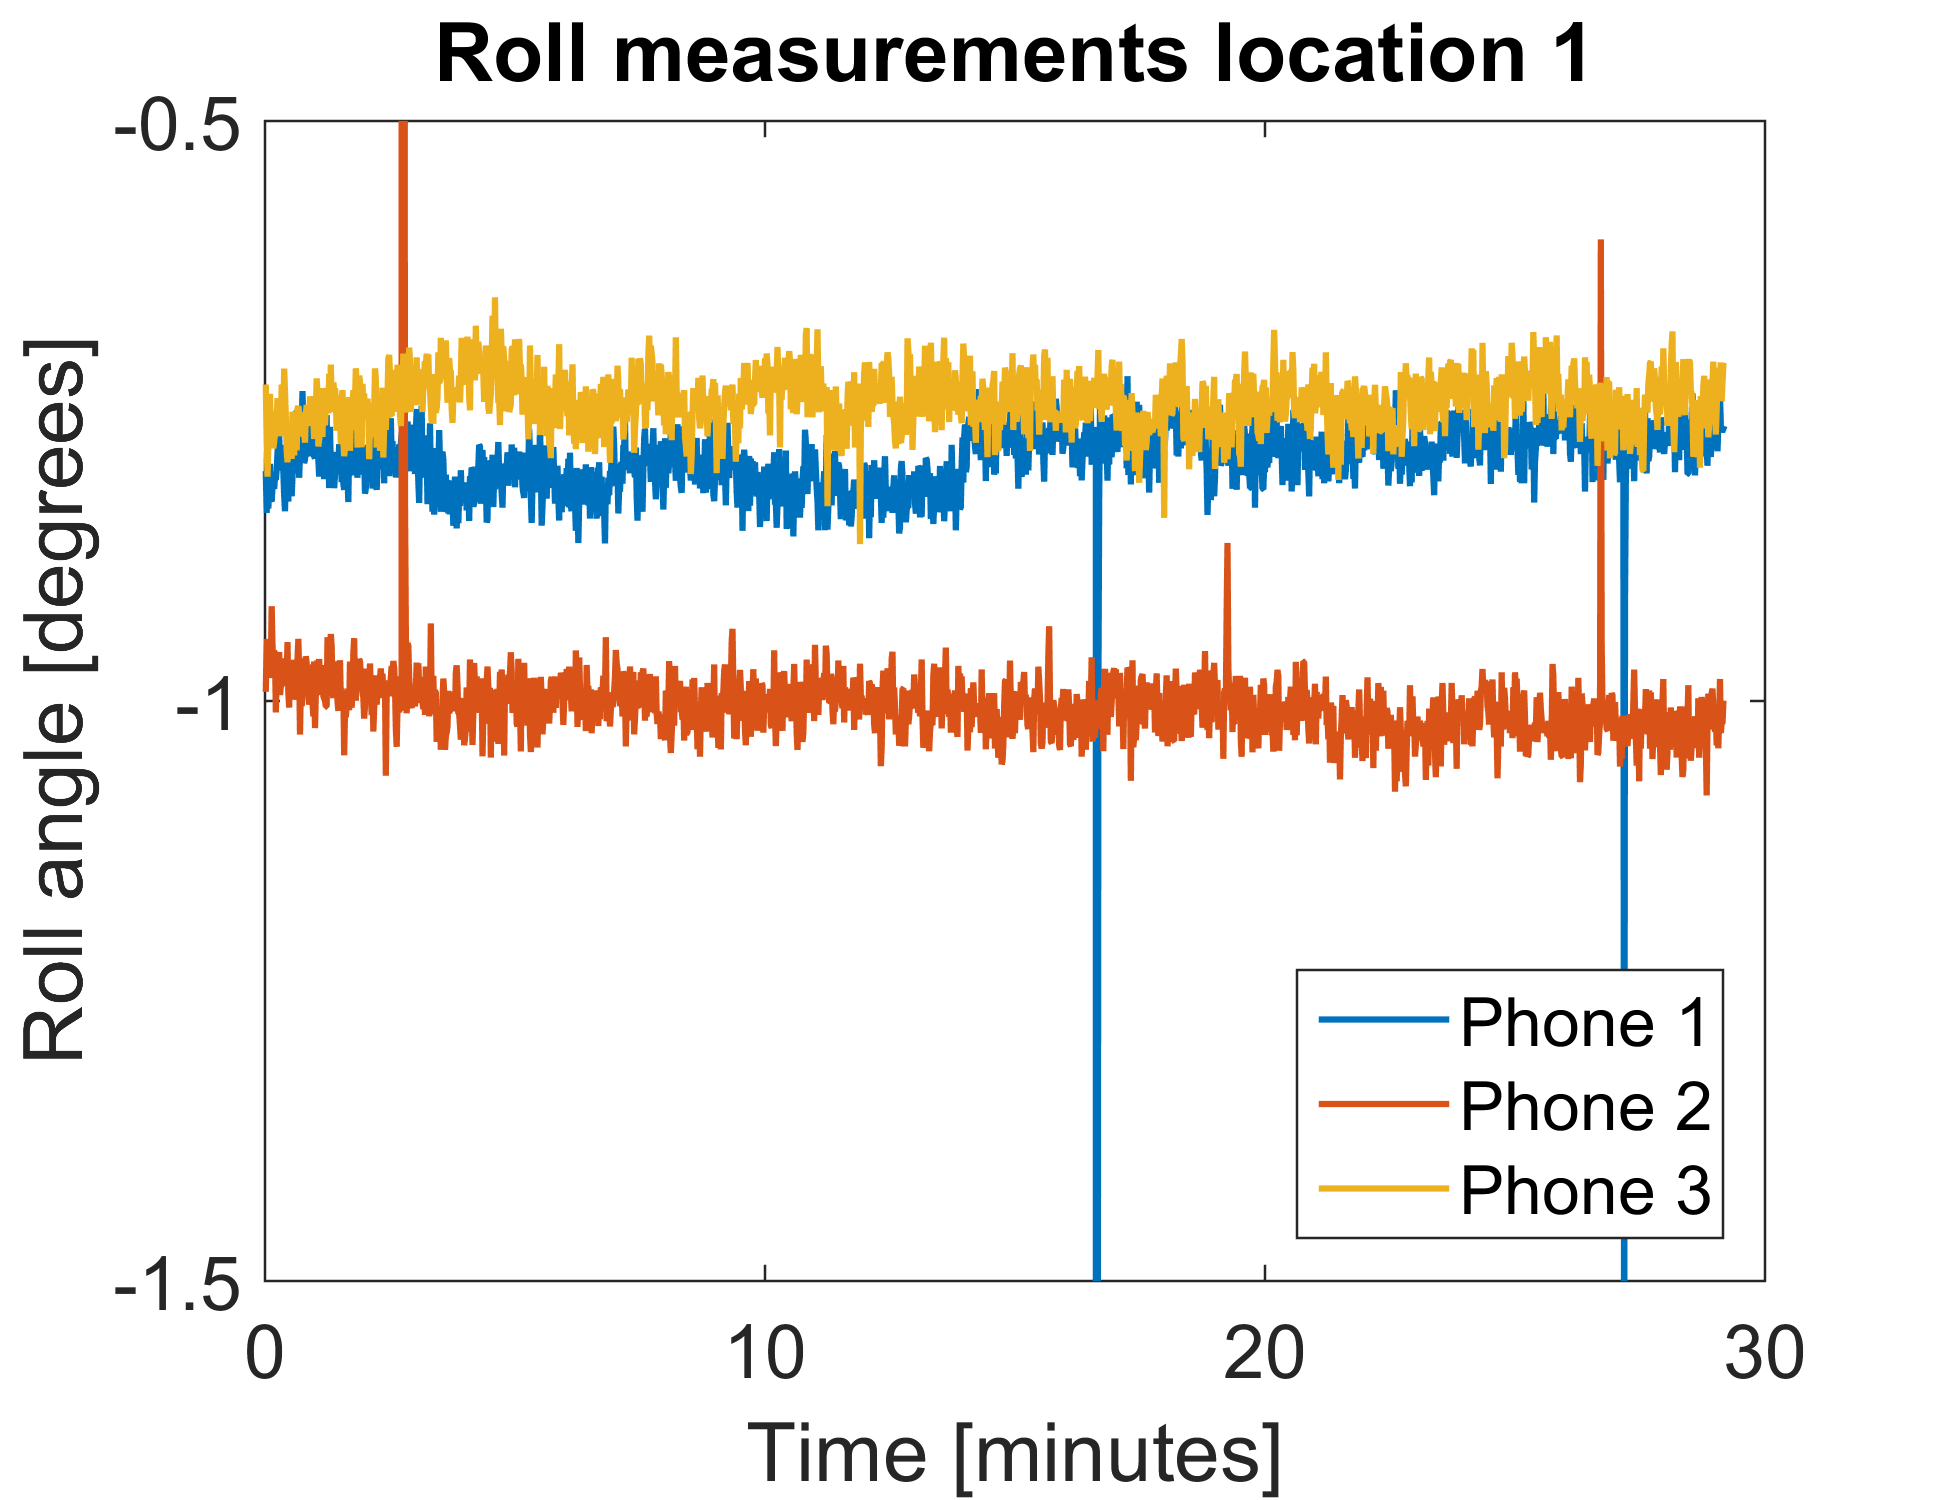
\includegraphics[width=\textwidth]{figures/orientation/ro_loc1}
		\caption{Roll angles for location 1.}
		\label{app:orientation_ro_loc1}
	\end{subfigure}
	\begin{subfigure}{0.33\textwidth}
		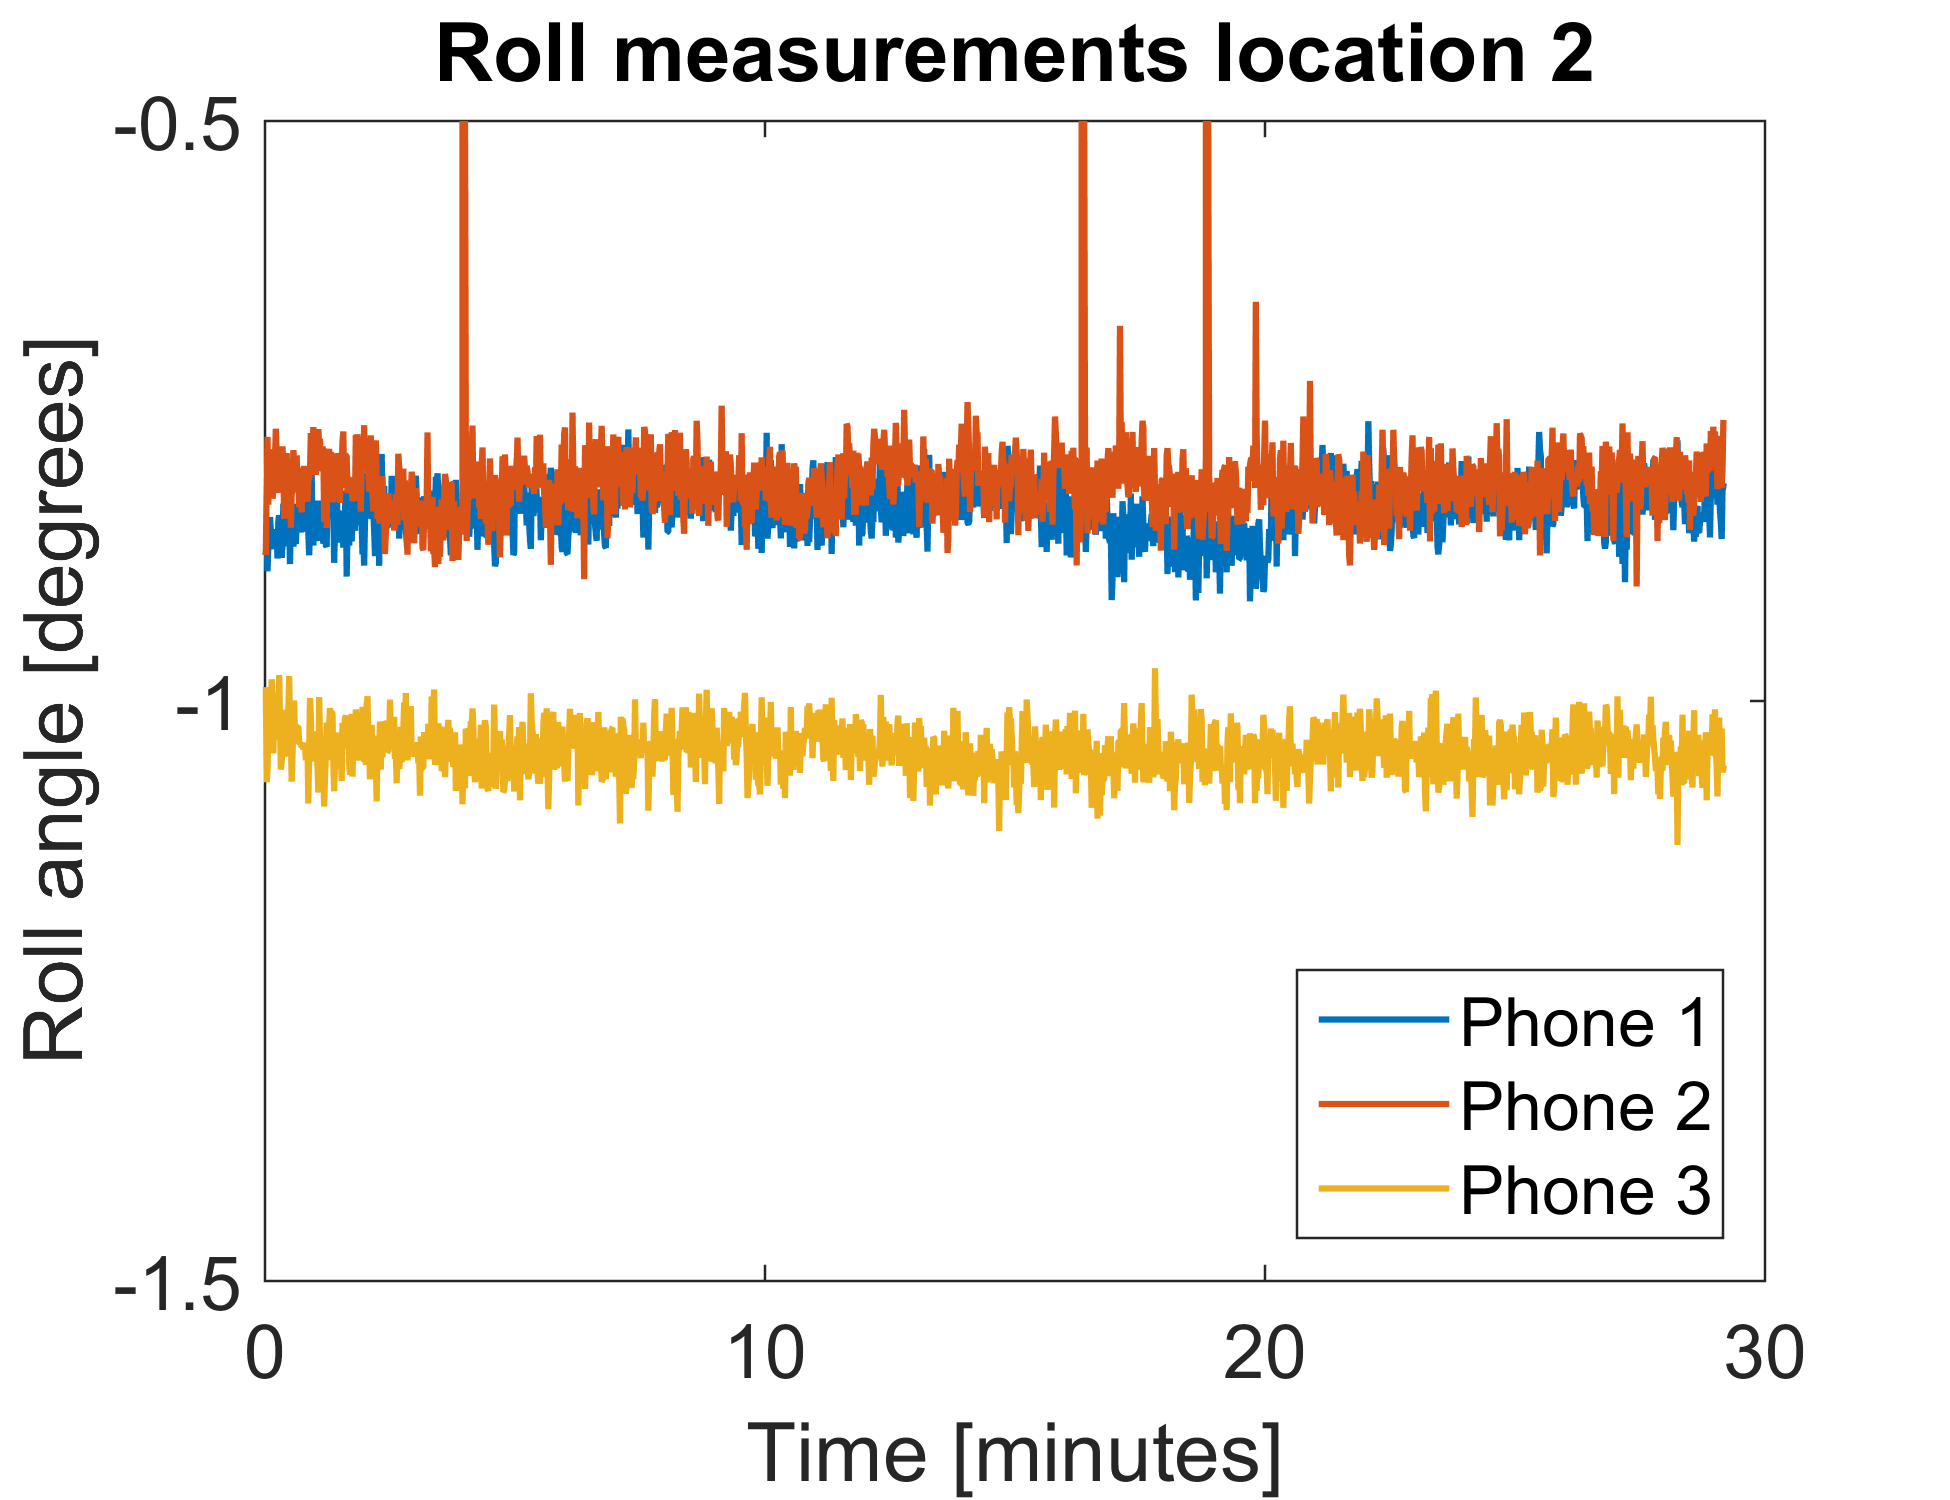
\includegraphics[width=\textwidth]{figures/orientation/ro_loc2}
		\caption{Roll angles for location 2.}
		\label{app:orientation_ro_loc2}
	\end{subfigure}
	\begin{subfigure}{0.33\textwidth}
		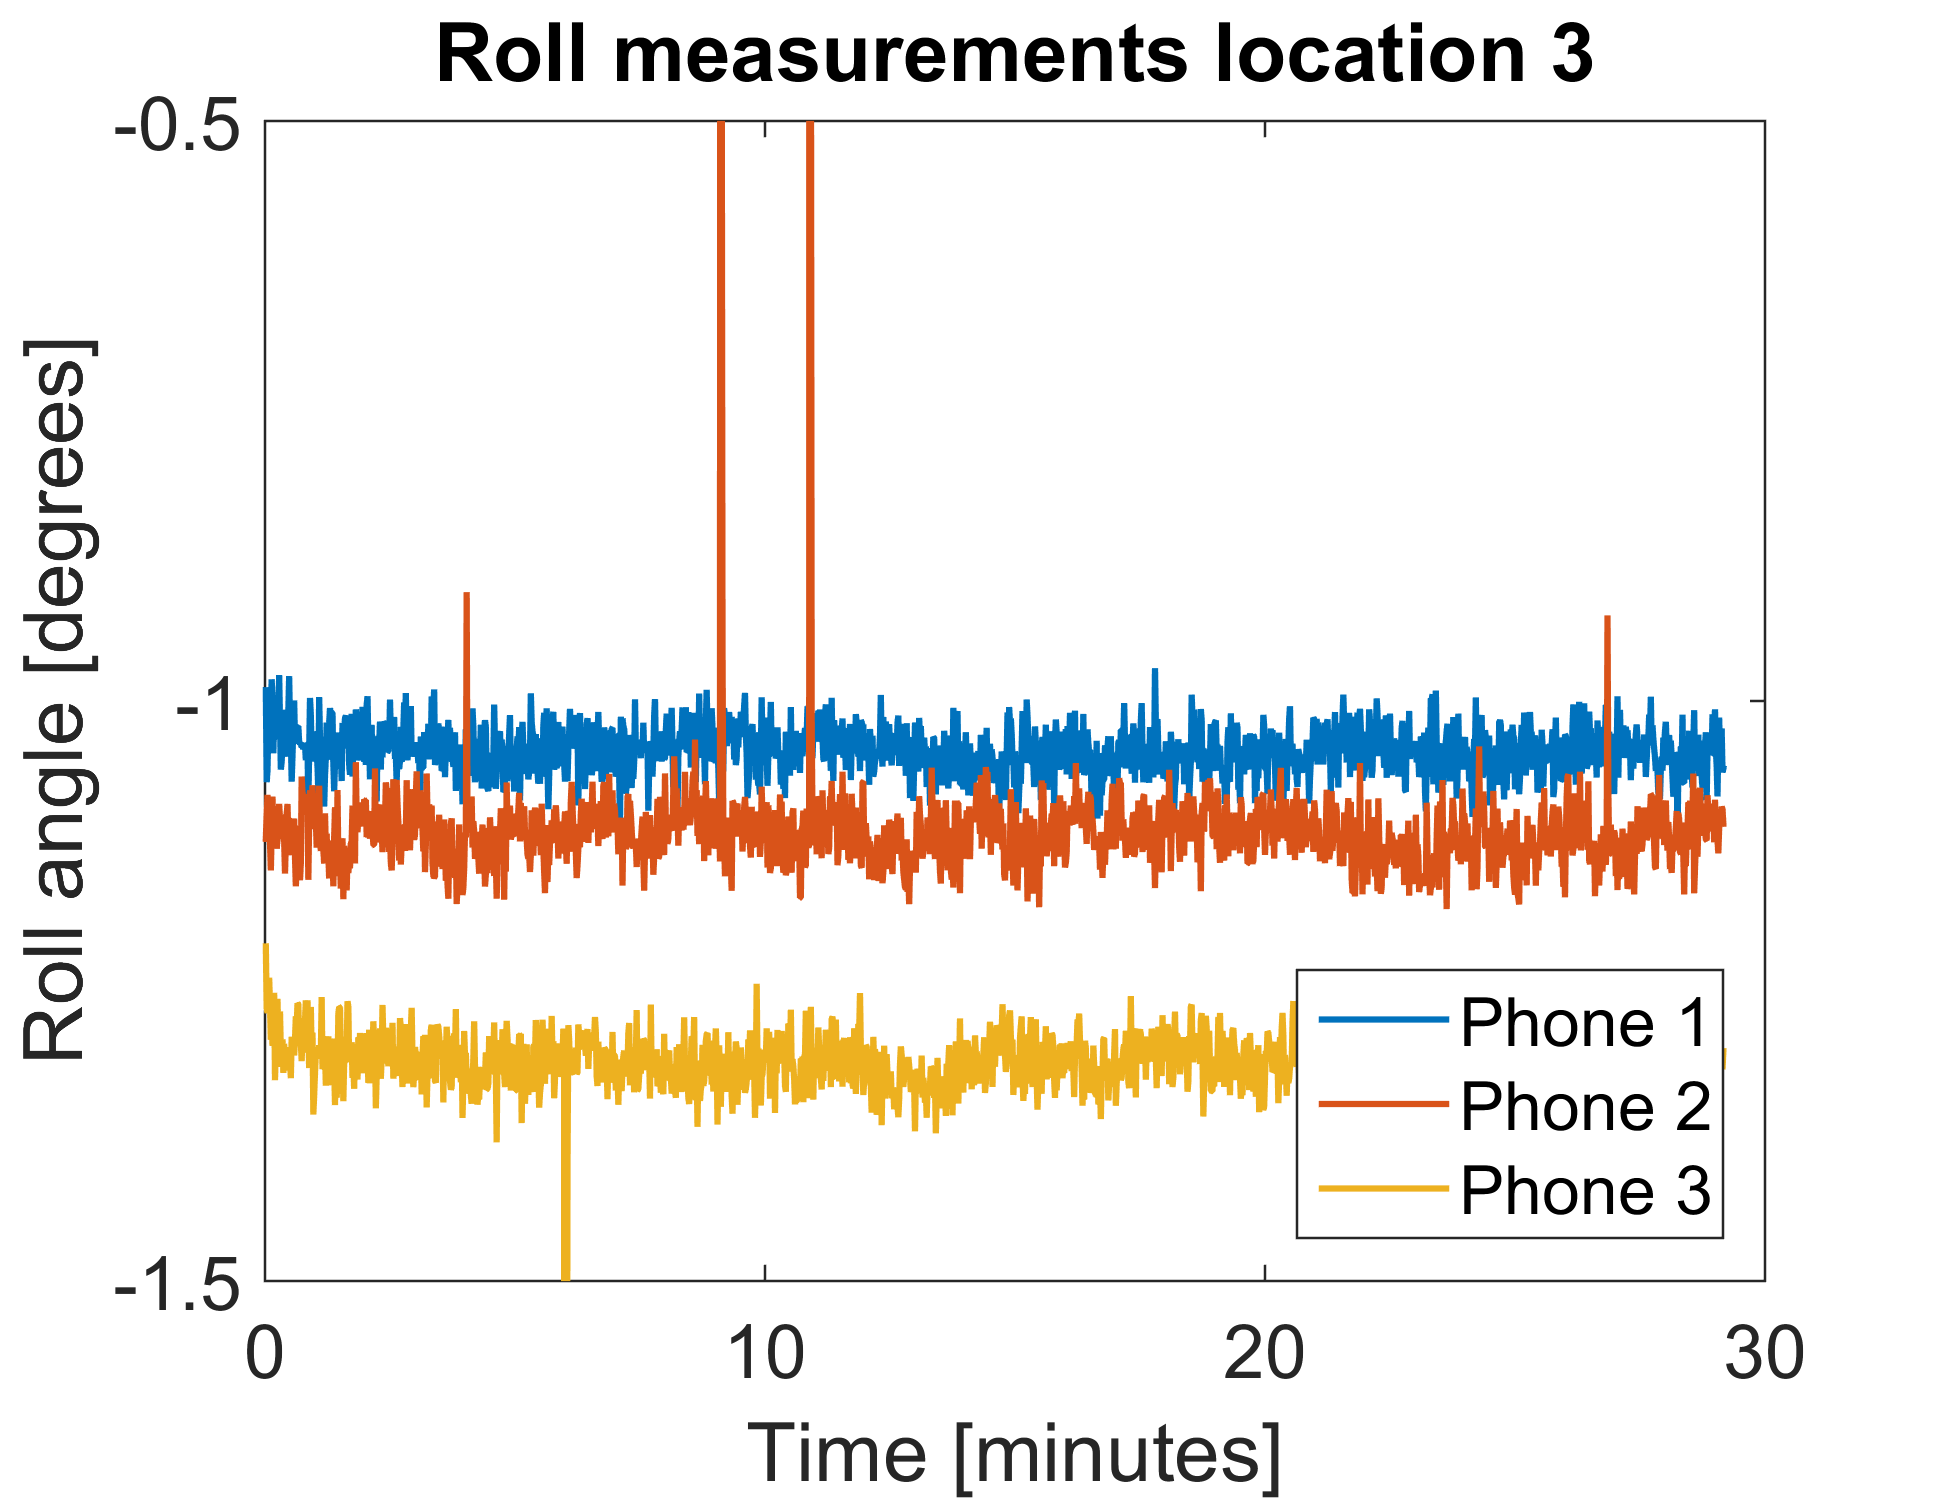
\includegraphics[width=\textwidth]{figures/orientation/ro_loc3}
		\caption{Roll angles for location 3.}
		\label{app:orientation_ro_loc3}
	\end{subfigure}
\end{adjustwidth}
\caption[Complete orientation measurement results.]{Complete measurement results for all orientation measurements performed.}
\label{app:orientation_total}
\end{figure}

\section{Time offset simulation}
\begin{figure}[h!]
\begin{adjustwidth}{-1in}{-1in}
\centering
	\begin{subfigure}{0.5\textwidth}
		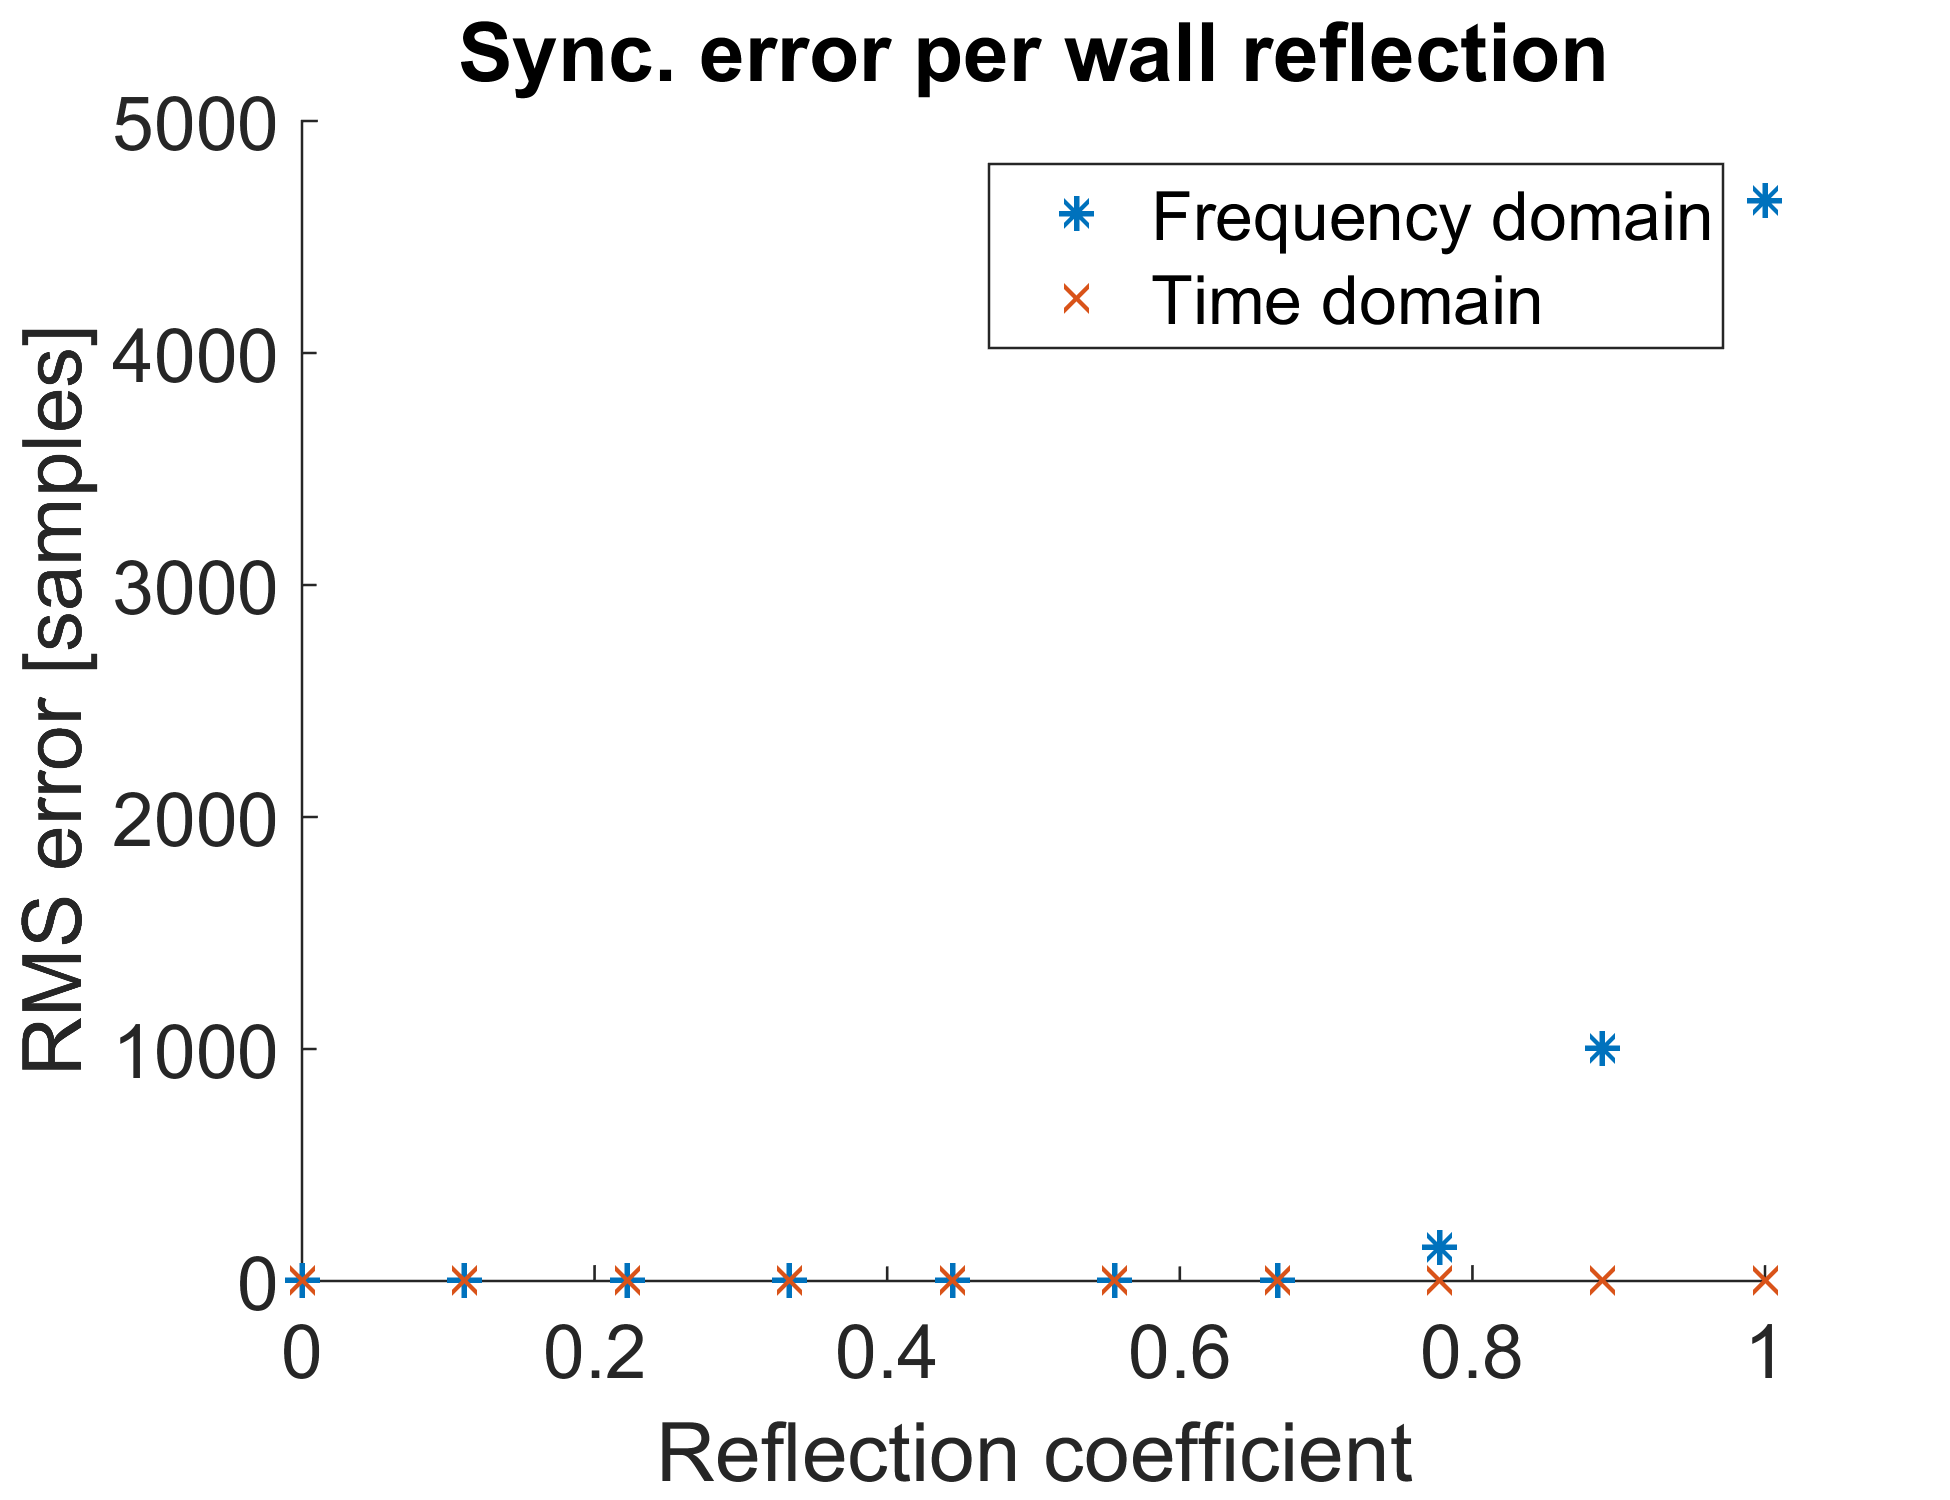
\includegraphics[width=\textwidth]{figures/sync-simulation/error-vs-reflection}
		\caption{Delay estimation error as a function of wall reflection.}
		\label{app:sync-simulation-reflection}
	\end{subfigure}
	\begin{subfigure}{0.5\textwidth}
		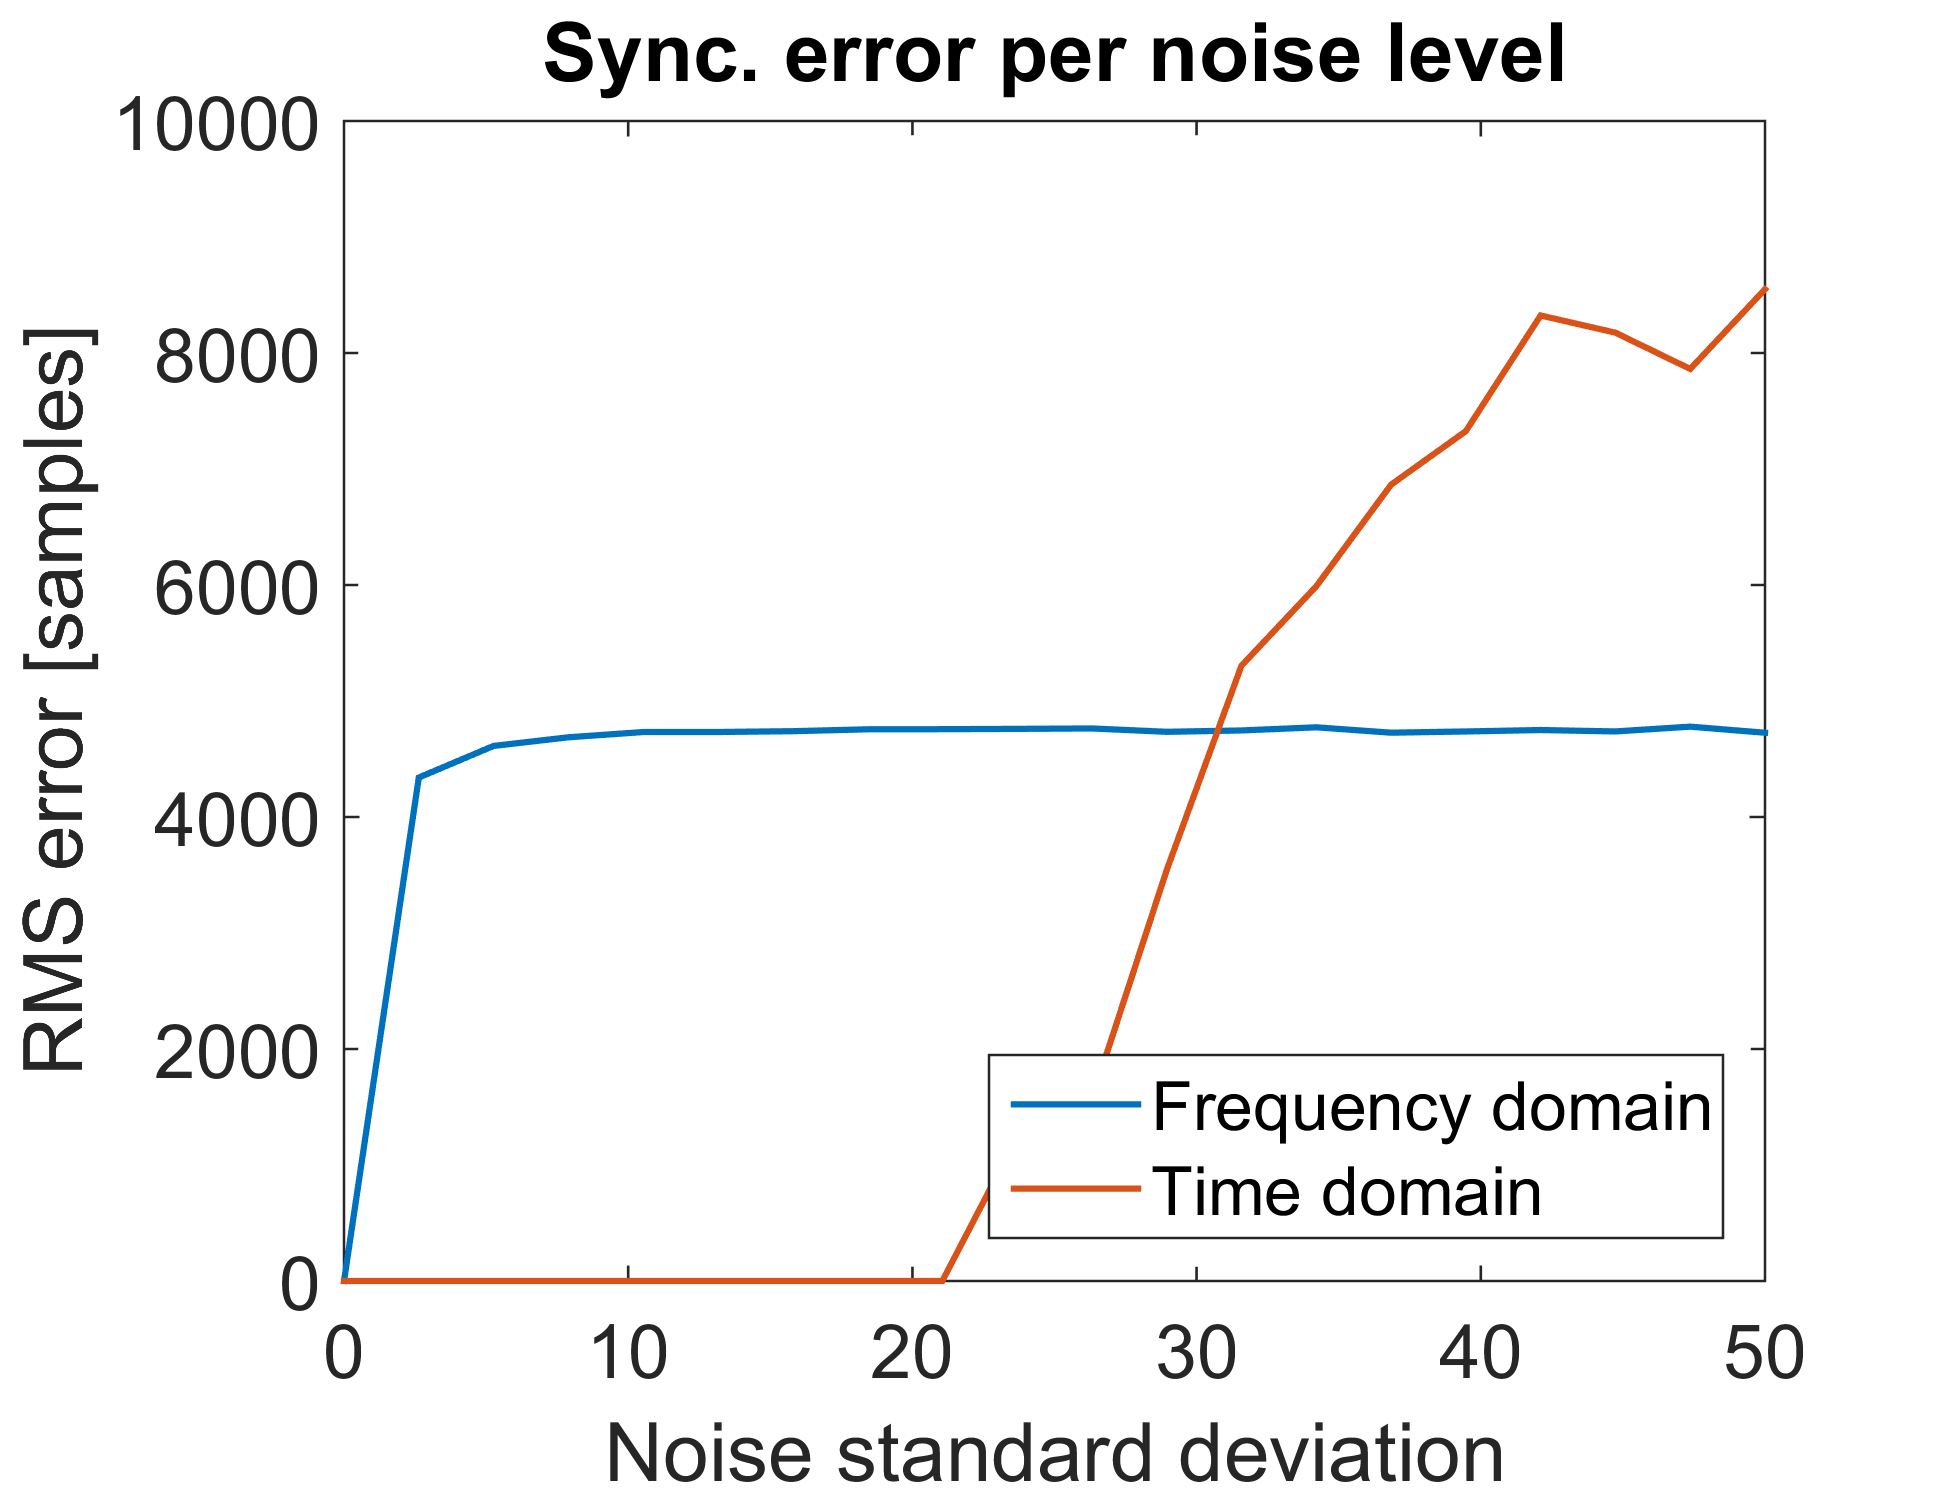
\includegraphics[width=\textwidth]{figures/sync-simulation/error-vs-noise}
		\caption{Delay estimation error as a function of noise power}
		\label{app:sync-simulation-noise}
	\end{subfigure}
	
	\begin{subfigure}{0.5\textwidth}
		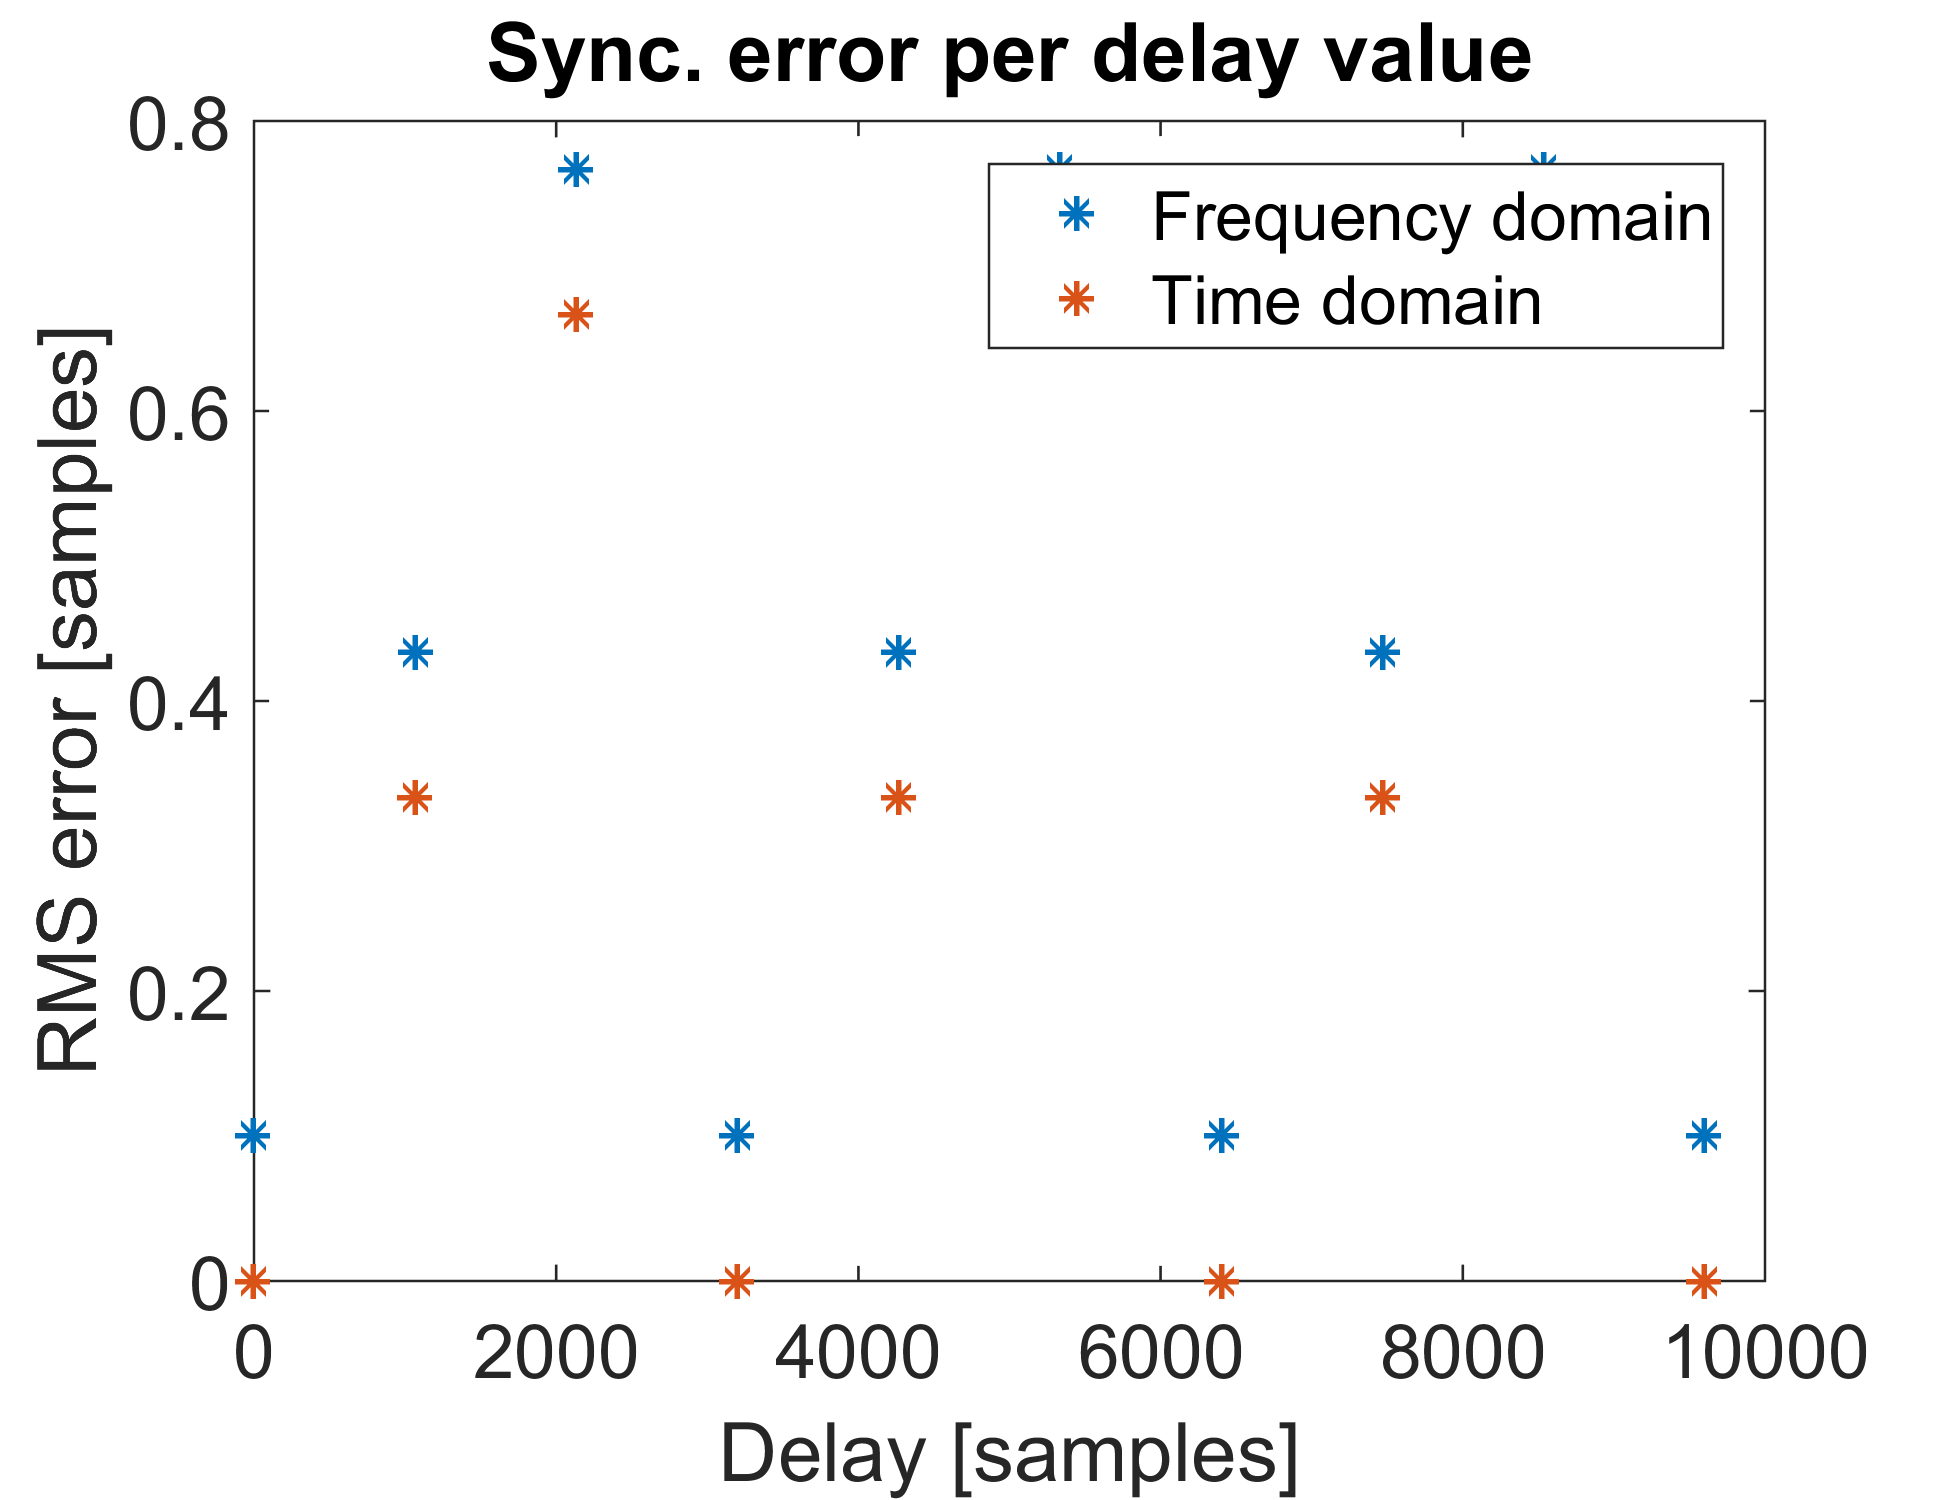
\includegraphics[width=\textwidth]{figures/sync-simulation/error-vs-delay}
		\caption{Delay estimation error as a function of inserted delay}
		\label{app:sync-simulation-delay}
	\end{subfigure}
	\begin{subfigure}{0.5\textwidth}
	~
	\end{subfigure}
\end{adjustwidth}
\caption[Full TD and FD synchronization simulation results.]{Simulated results for TD and FD synchronization algorithm. The time-domain algorithm performs better under nearly all circumstances.}
\label{app:sync-simulation}
\end{figure}

	
\section{Sampling rate offset measurements}
\begin{figure}[H]
\begin{adjustwidth}{-1in}{-1in}
\centering
	\begin{subfigure}{0.5\textwidth}
		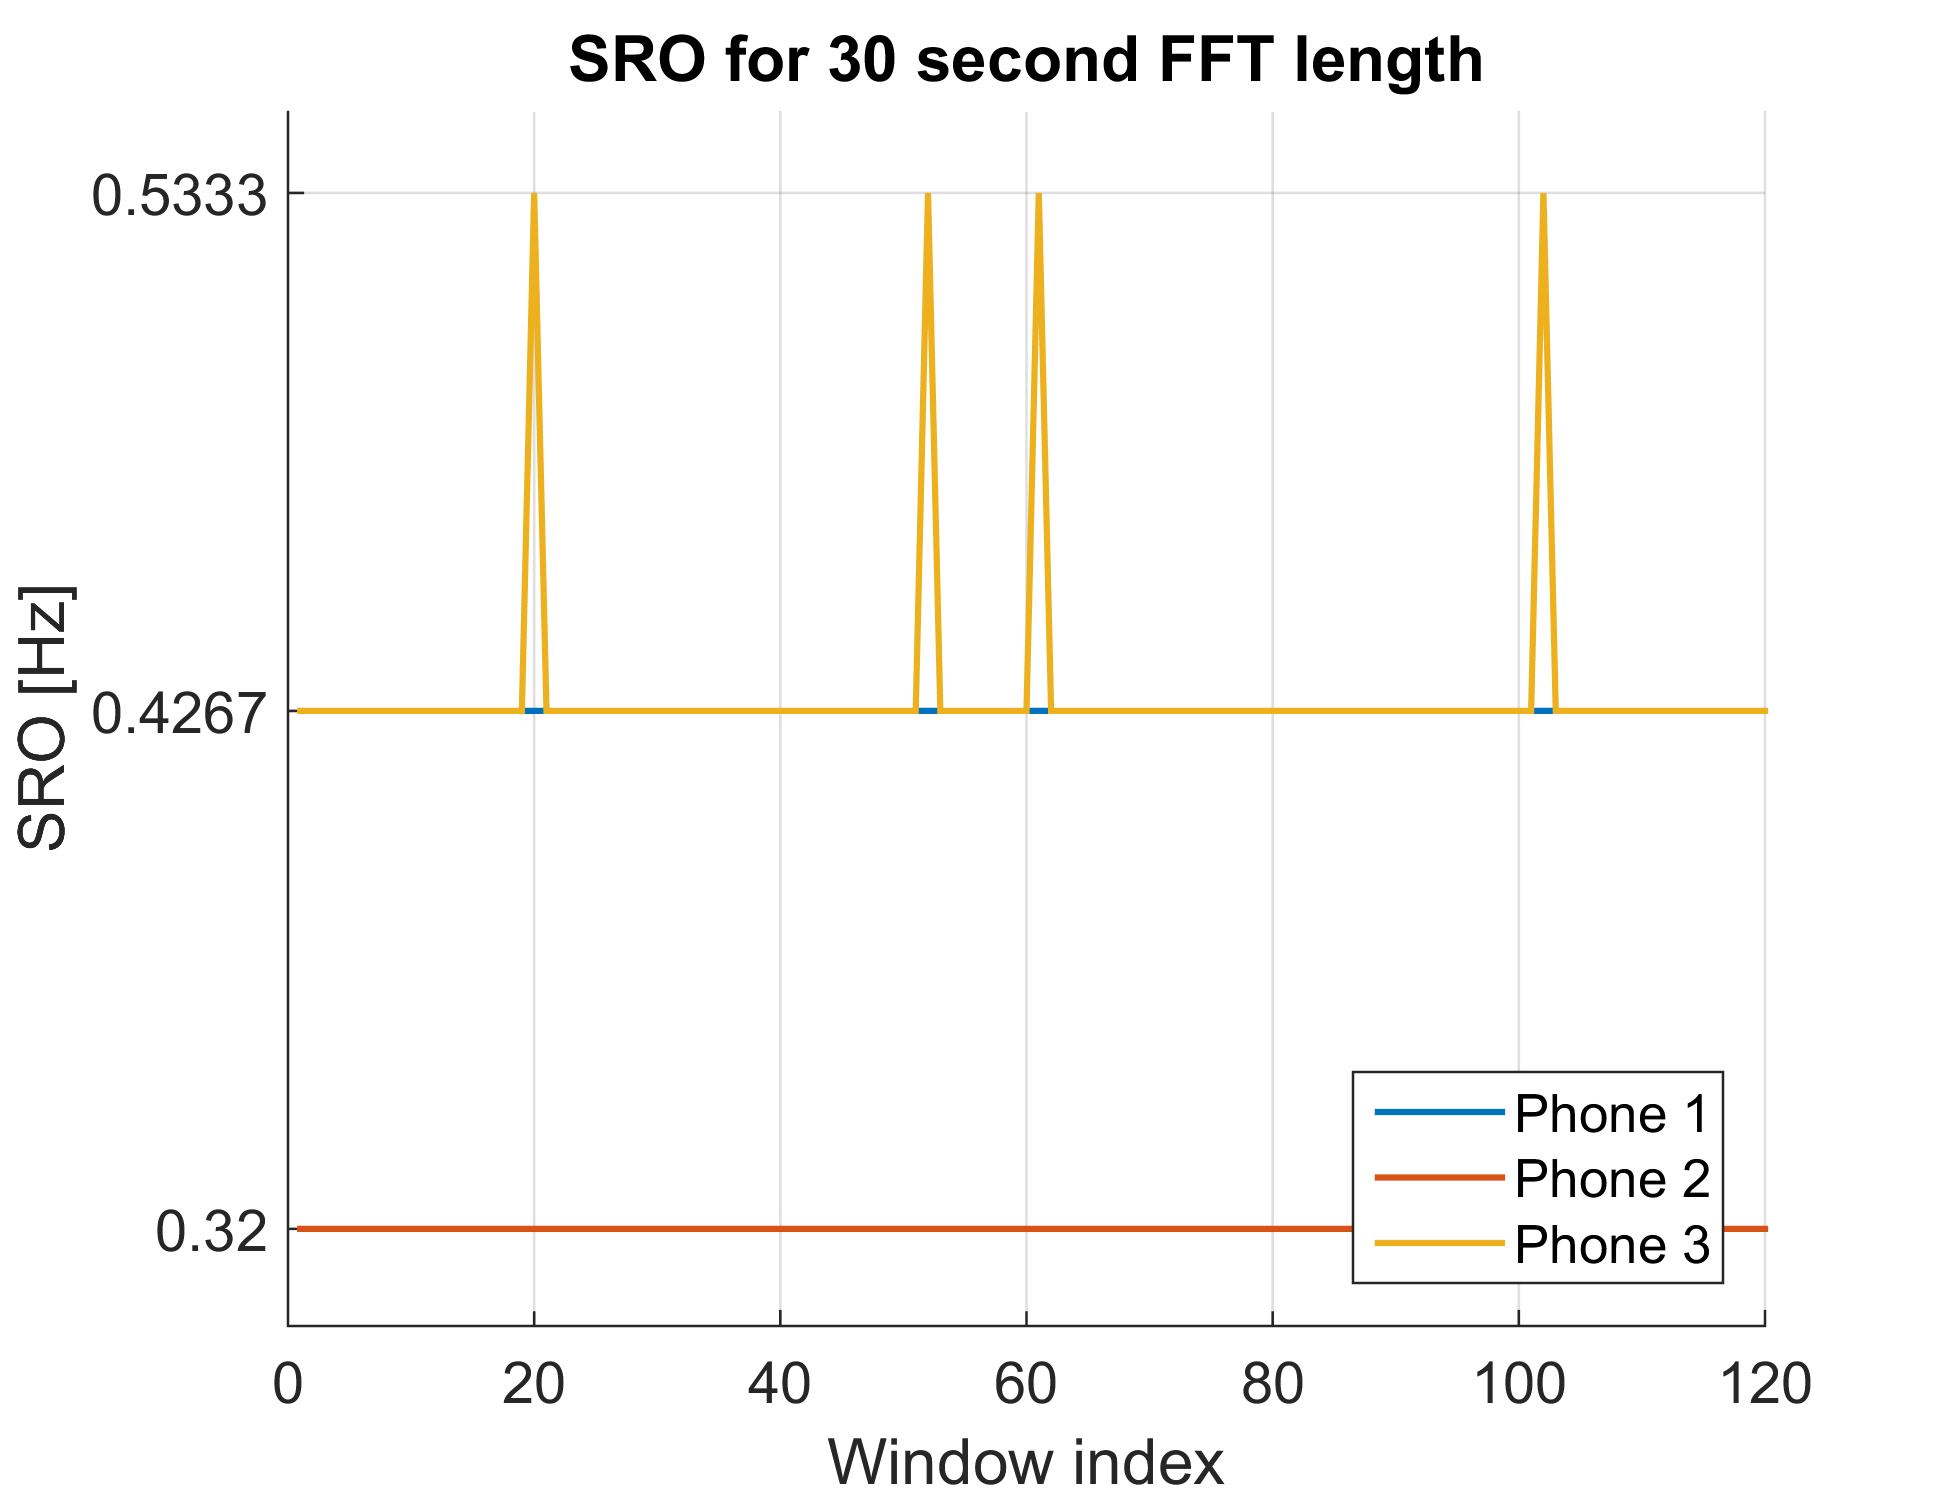
\includegraphics[width=\textwidth]{figures/sro-measurement/sro-30sec}
		\caption{30 second FFT window, $\Delta f=3.3~\mathrm{mHz}$.}
		\label{app:sro_30sec}
	\end{subfigure}
	\begin{subfigure}{0.5\textwidth}
		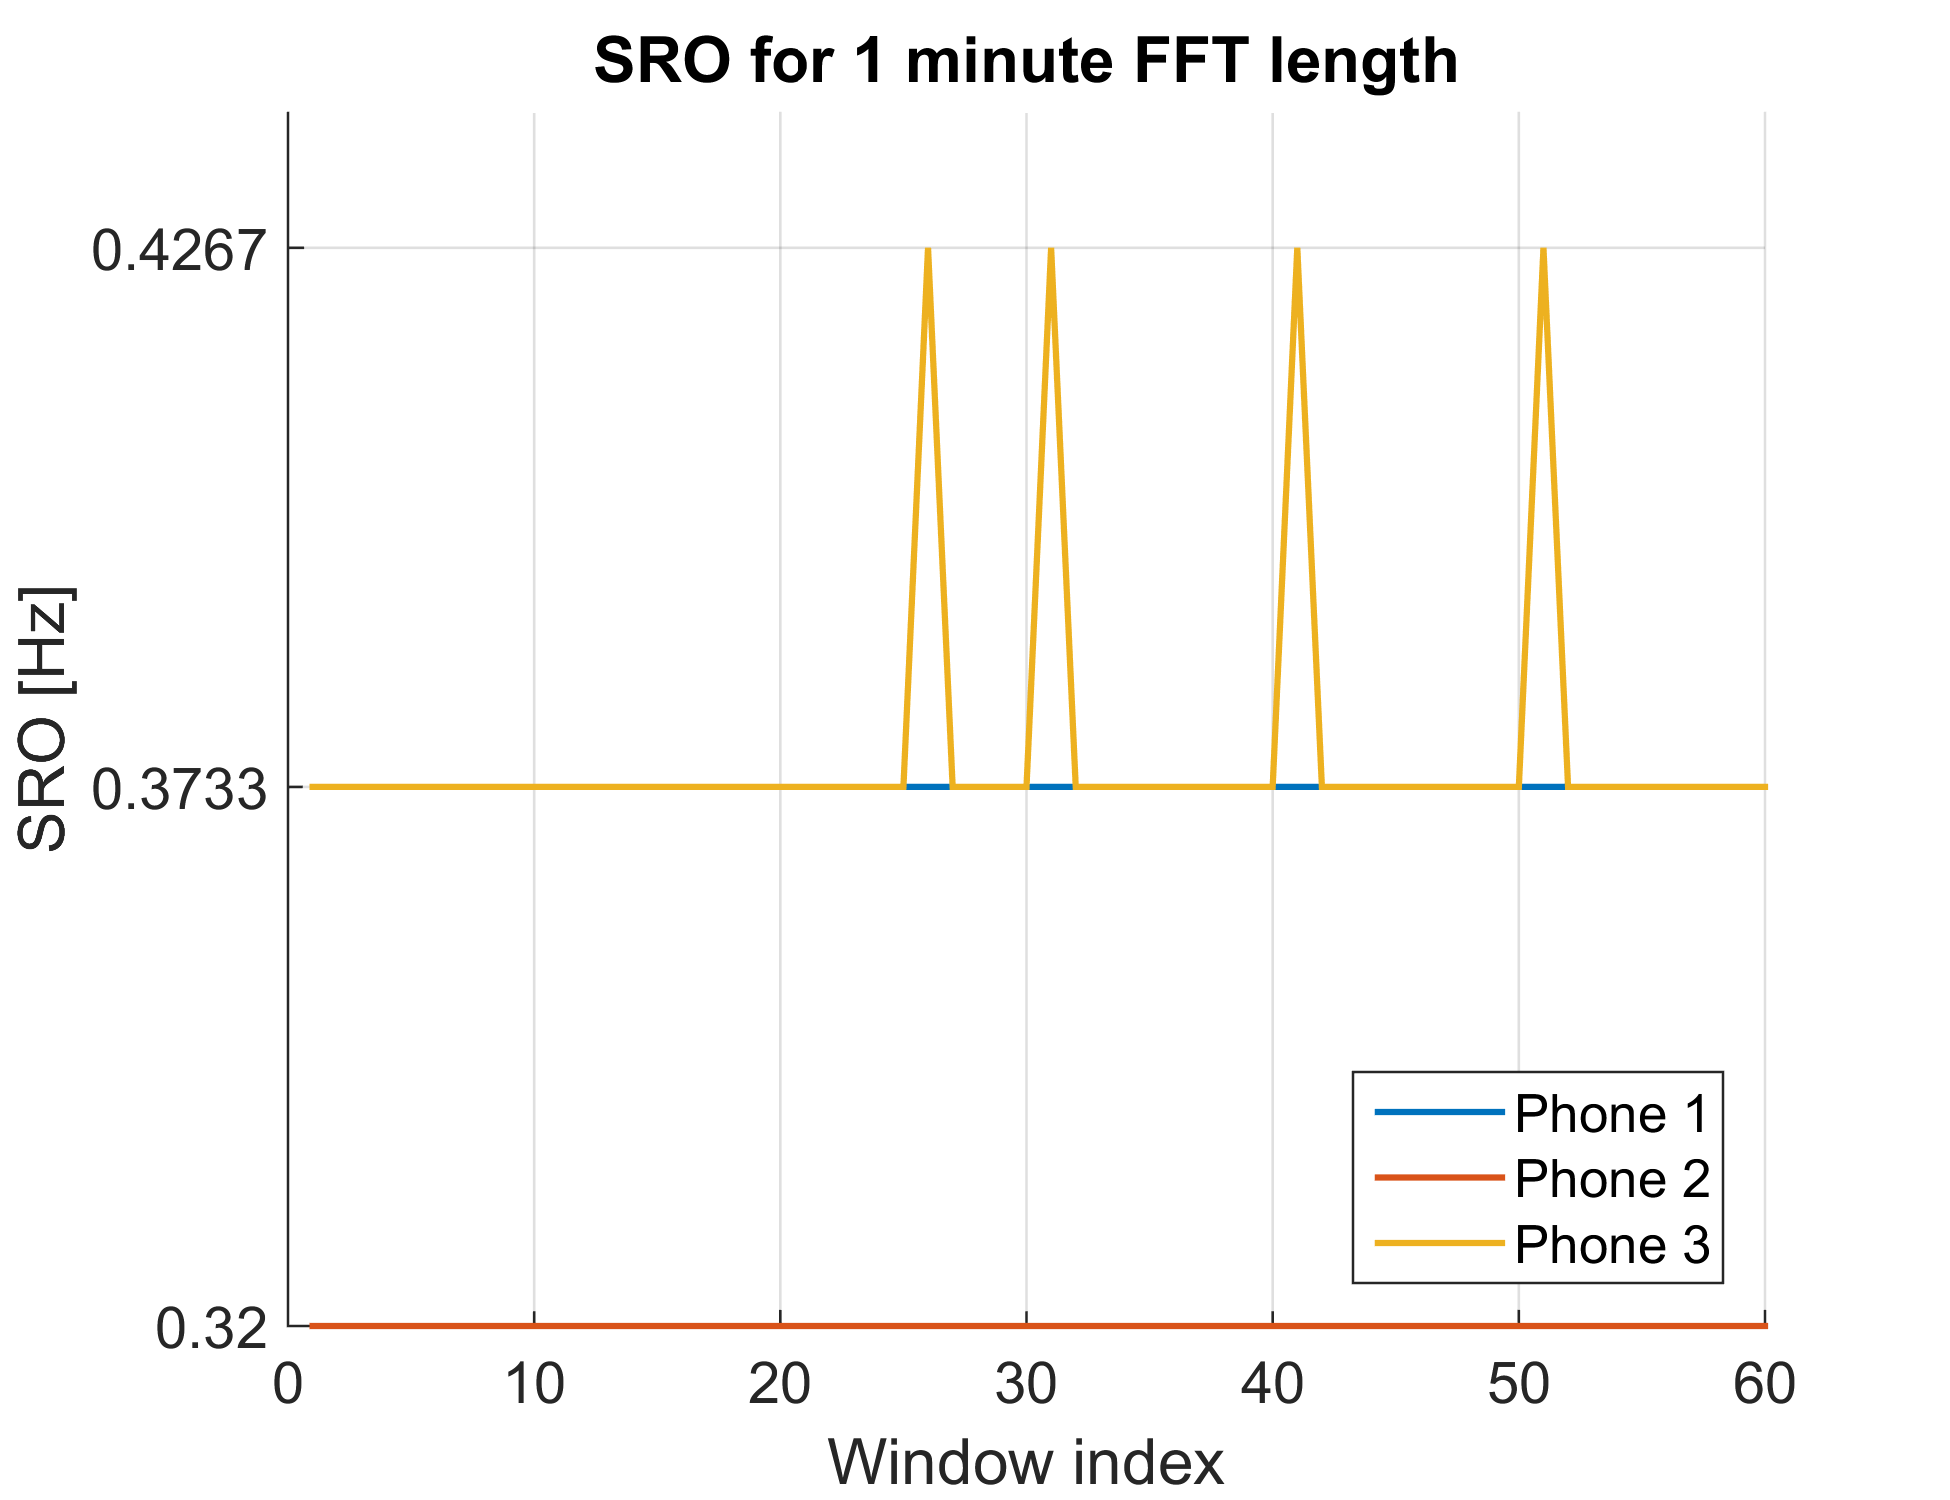
\includegraphics[width=\textwidth]{figures/sro-measurement/sro-1min}
		\caption{One minute FFT window, $\Delta f=6.6~\mathrm{mHz}$}
		\label{app:sro_1min}
	\end{subfigure}
	
	\vspace{10pt}
	\begin{subfigure}{0.5\textwidth}
		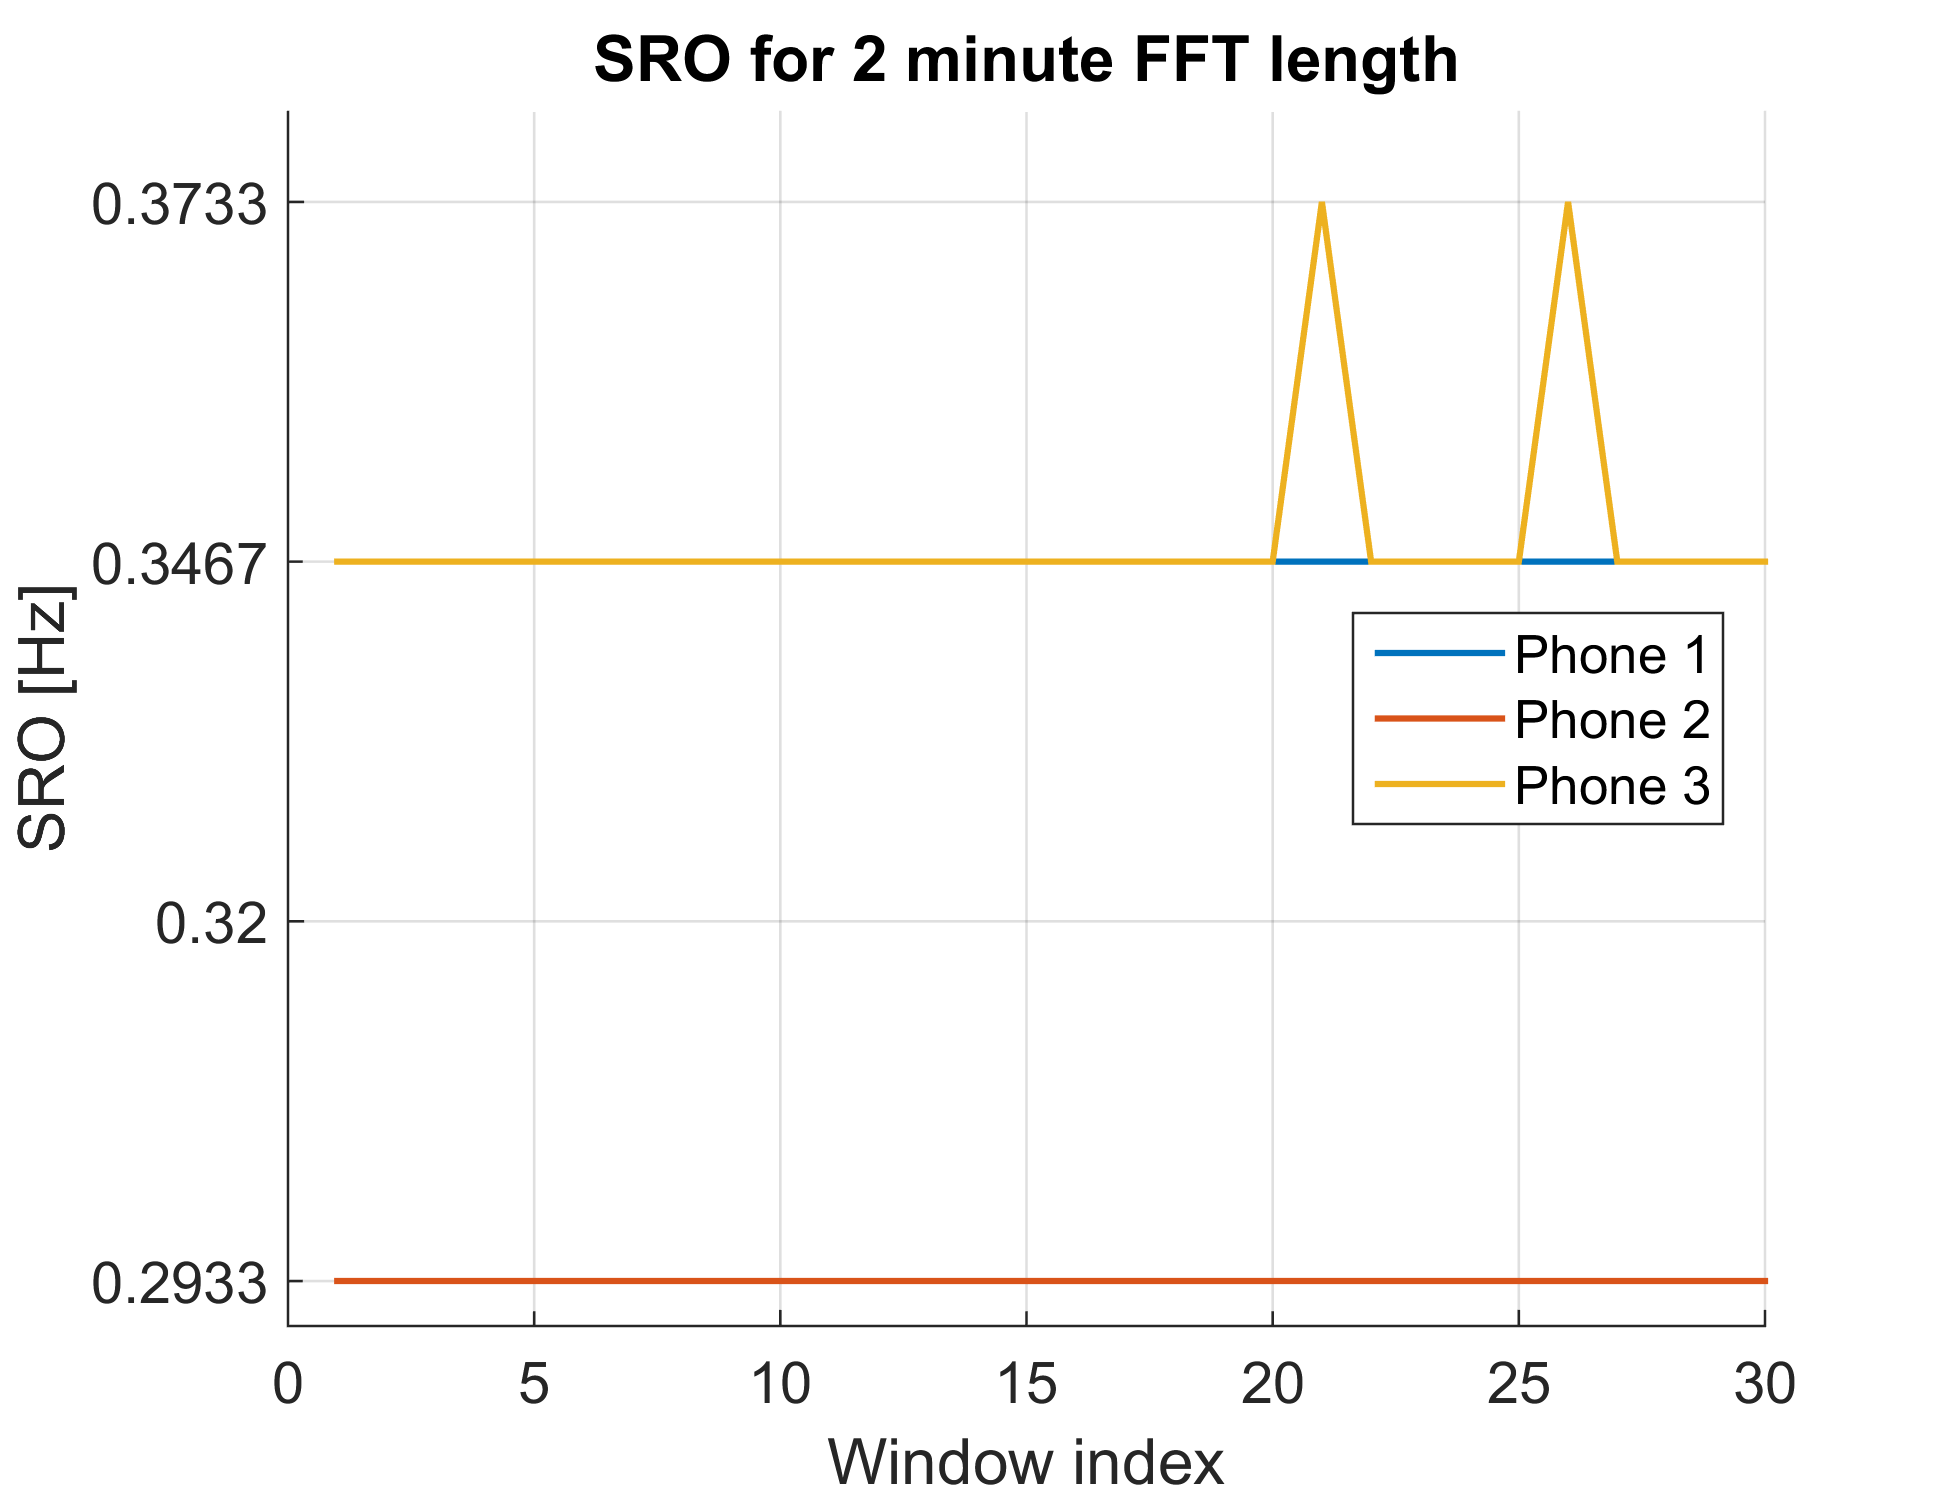
\includegraphics[width=\textwidth]{figures/sro-measurement/sro-2min}
		\caption{2 minute FFT window, $\Delta f=13.2~\mathrm{mHz}$.}
		\label{app:sro_2min}
	\end{subfigure}
	\begin{subfigure}{0.5\textwidth}
		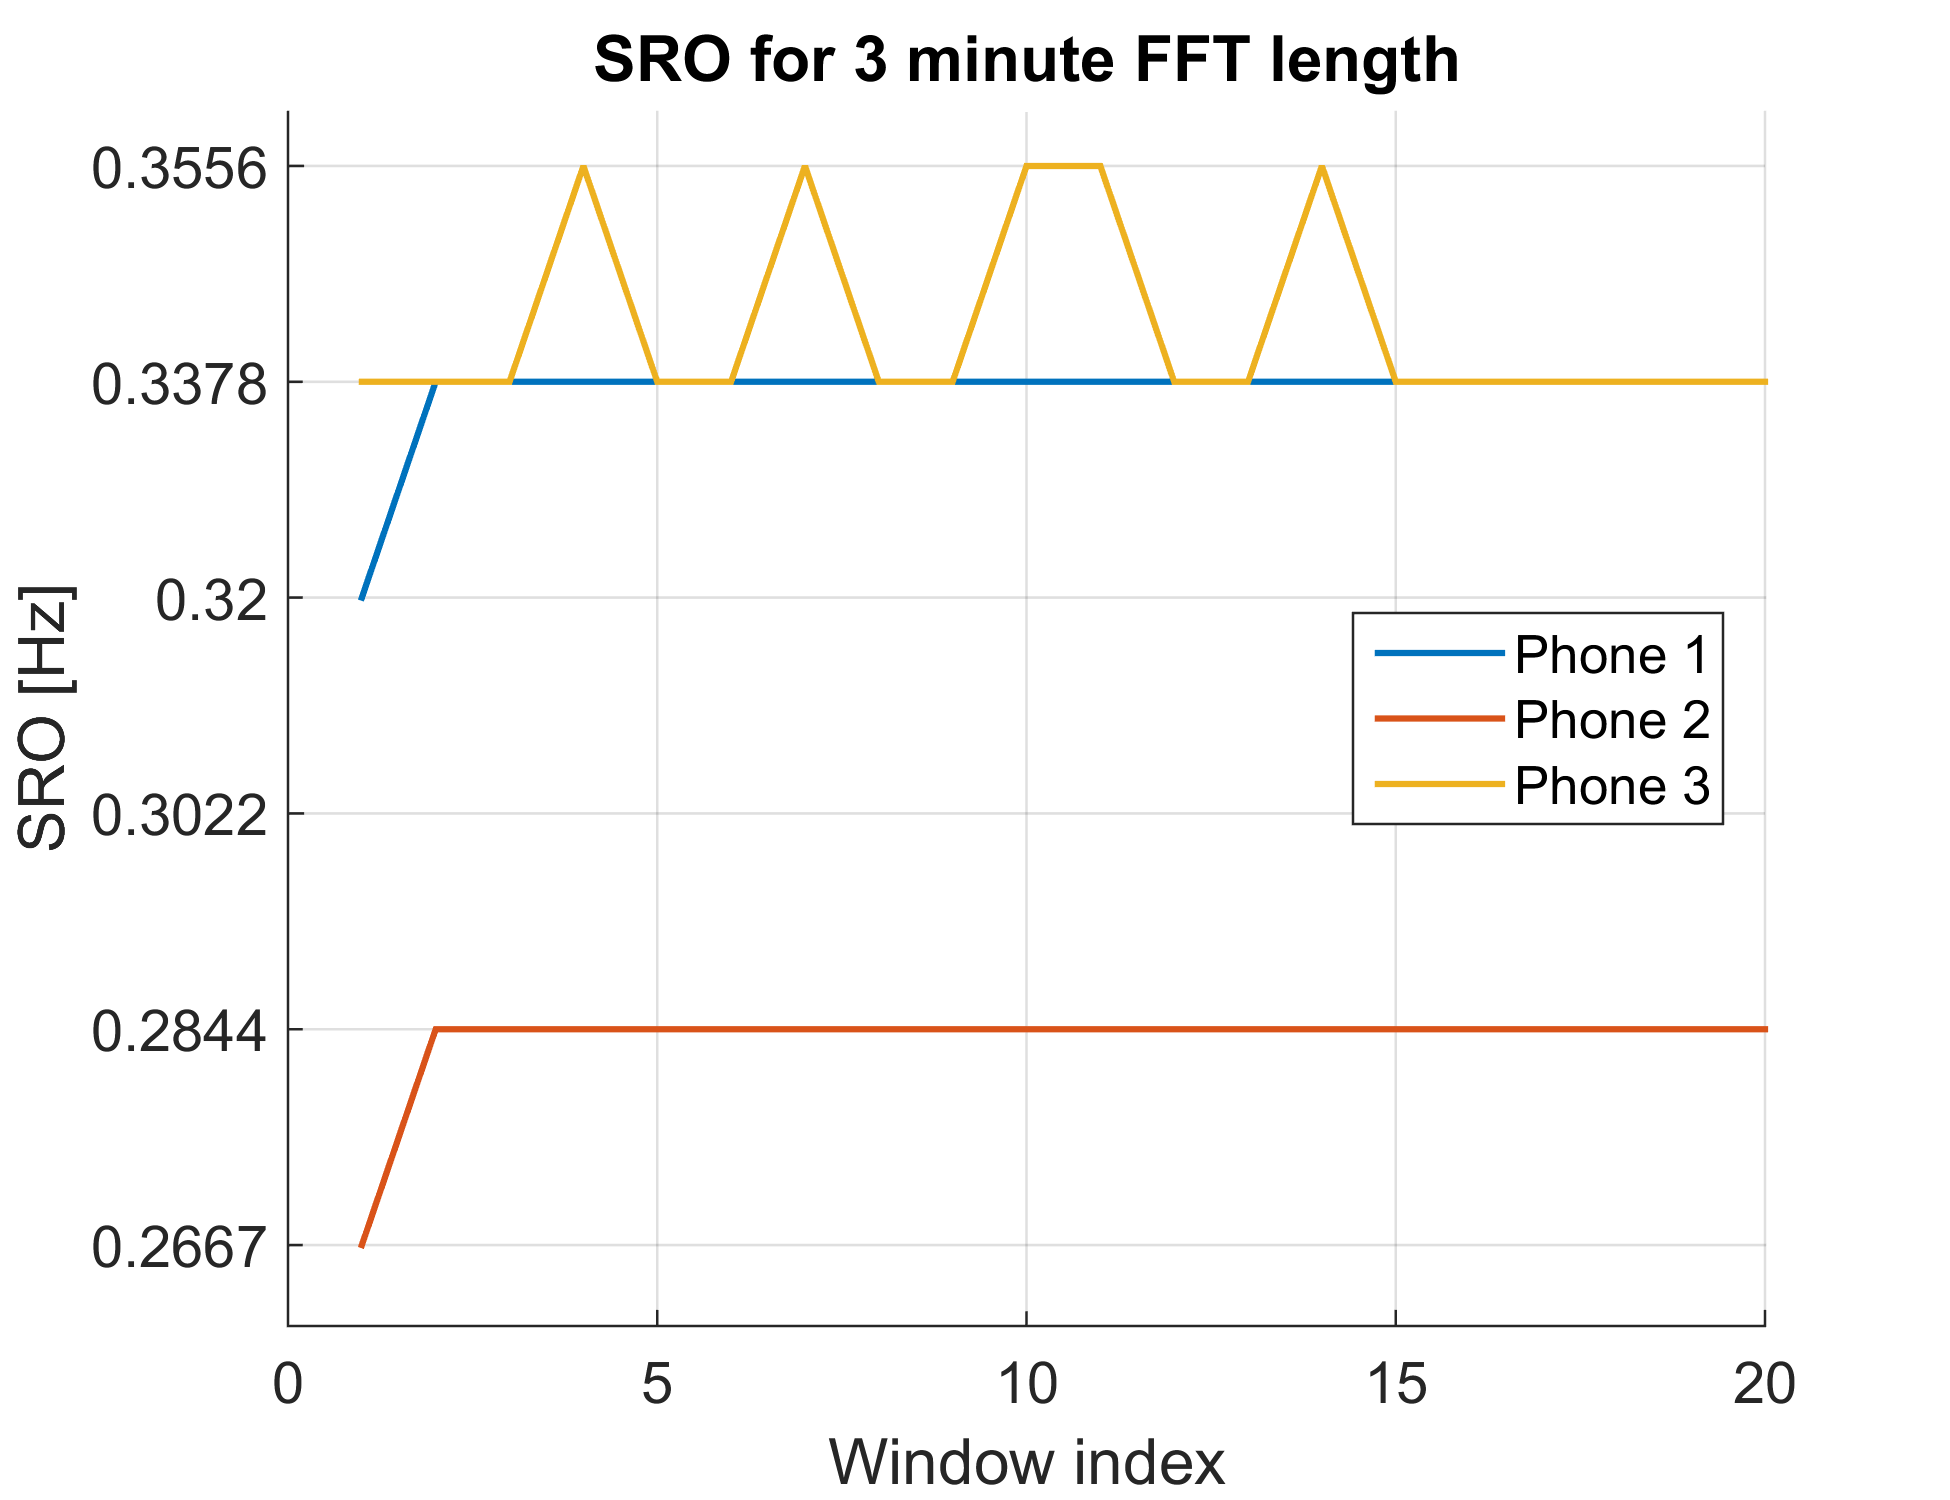
\includegraphics[width=\textwidth]{figures/sro-measurement/sro-3min}
		\caption{3 minute FFT window, $\Delta f=19.8~\mathrm{mHz}$.}
		\label{app:sro_3min}
	\end{subfigure}
	
	\vspace{10pt}
	\begin{subfigure}{0.5\textwidth}
		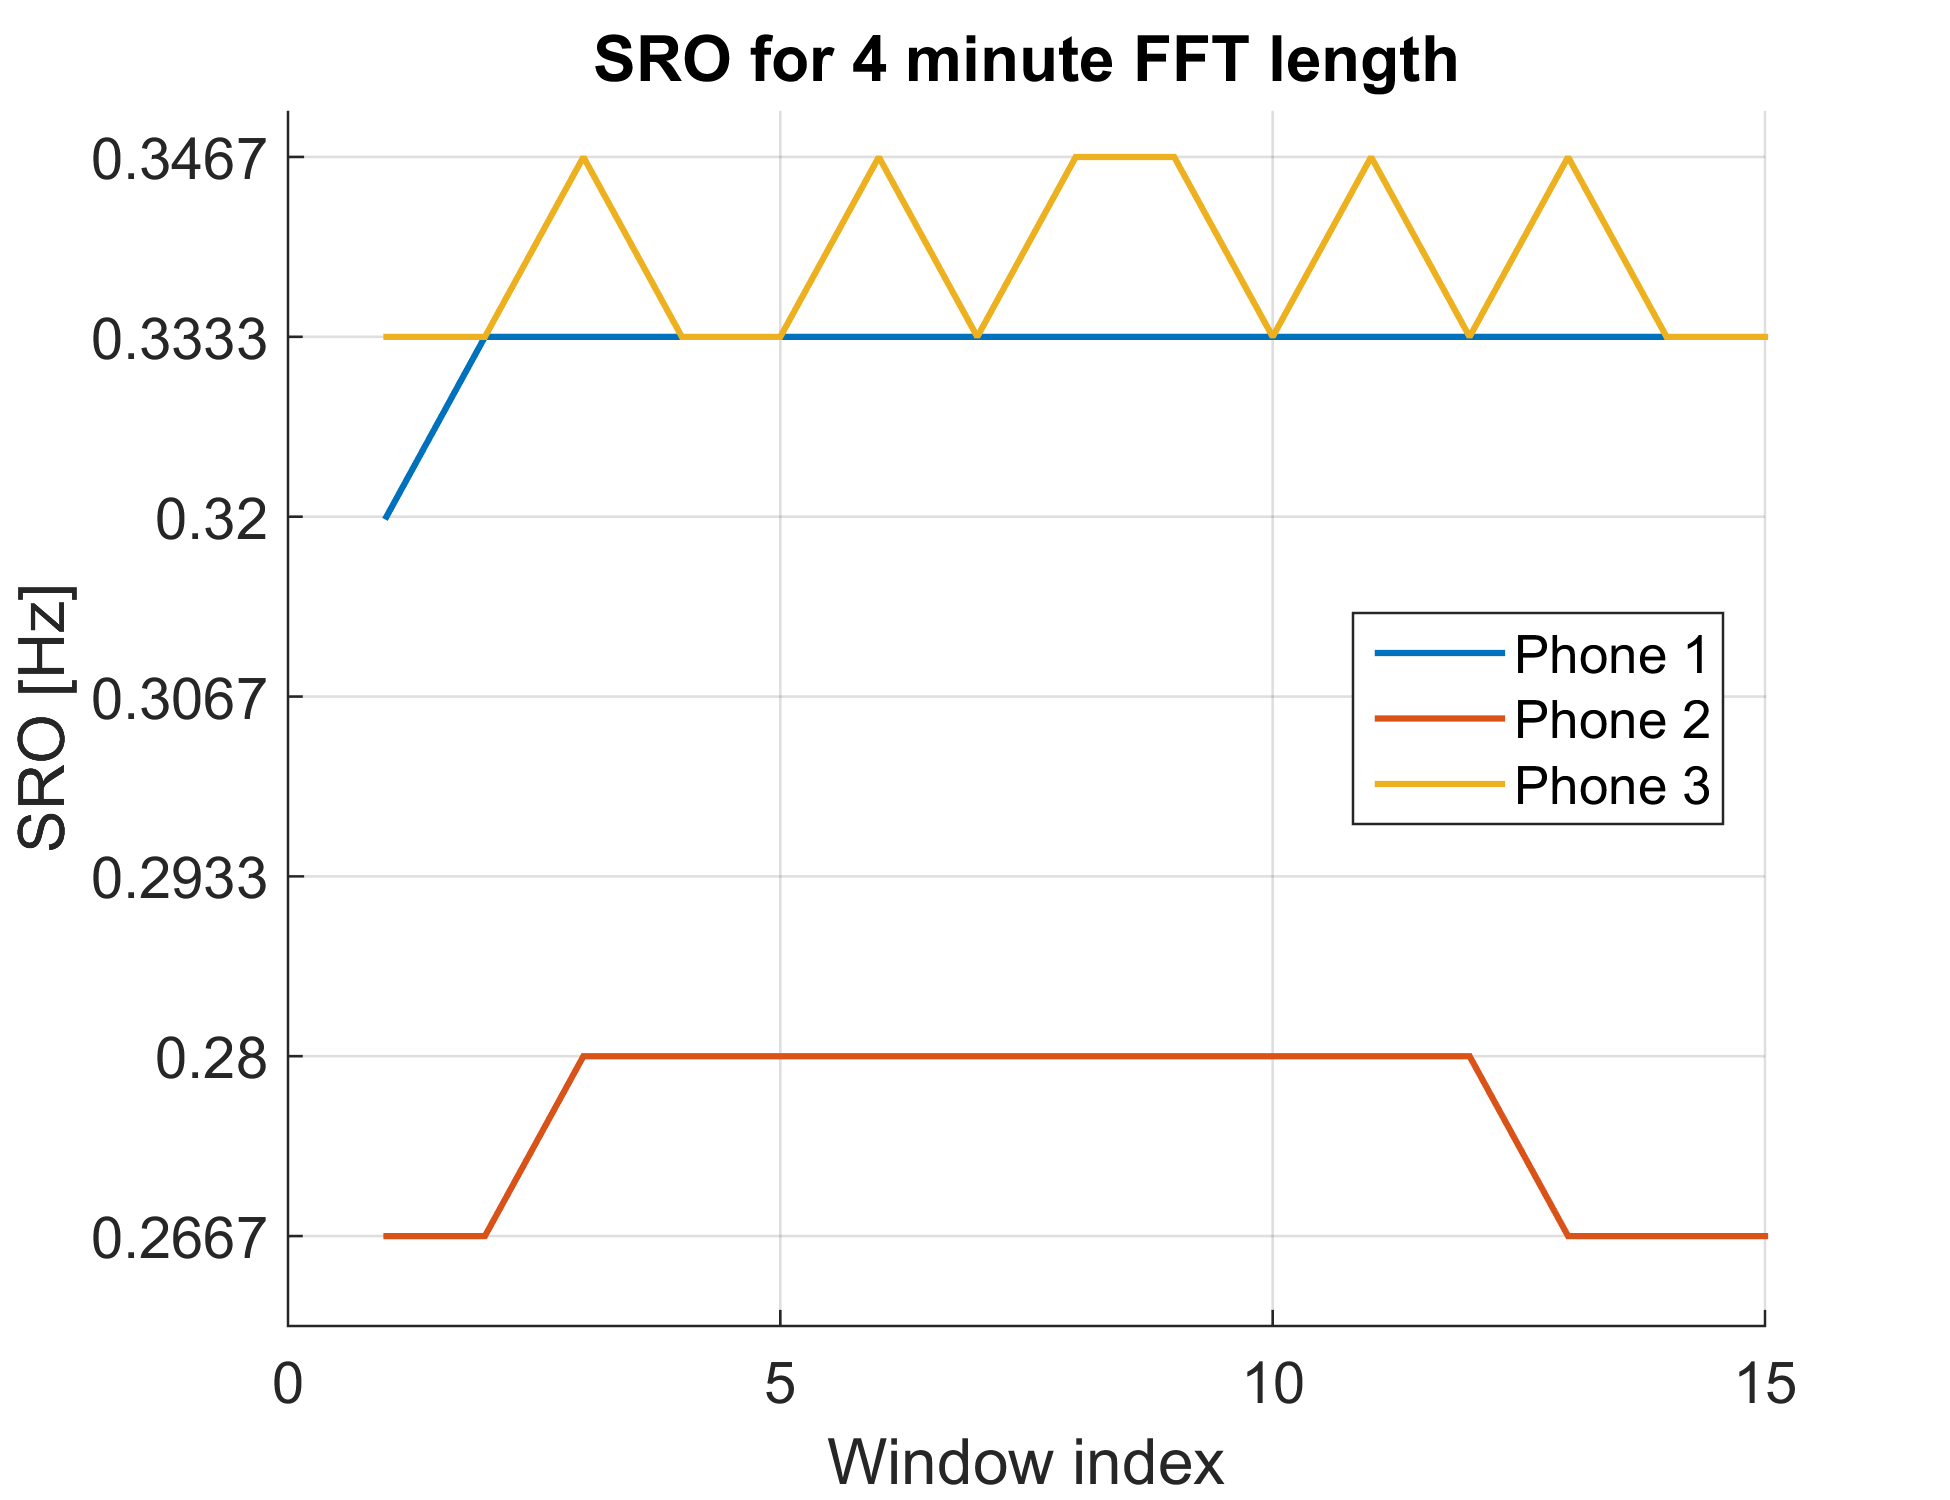
\includegraphics[width=\textwidth]{figures/sro-measurement/sro-4min}
		\caption{4 minute FFT window, $\Delta f=26.4~\mathrm{mHz}$.}
		\label{app:sro_4min}
	\end{subfigure}
	\begin{subfigure}{0.5\textwidth}
		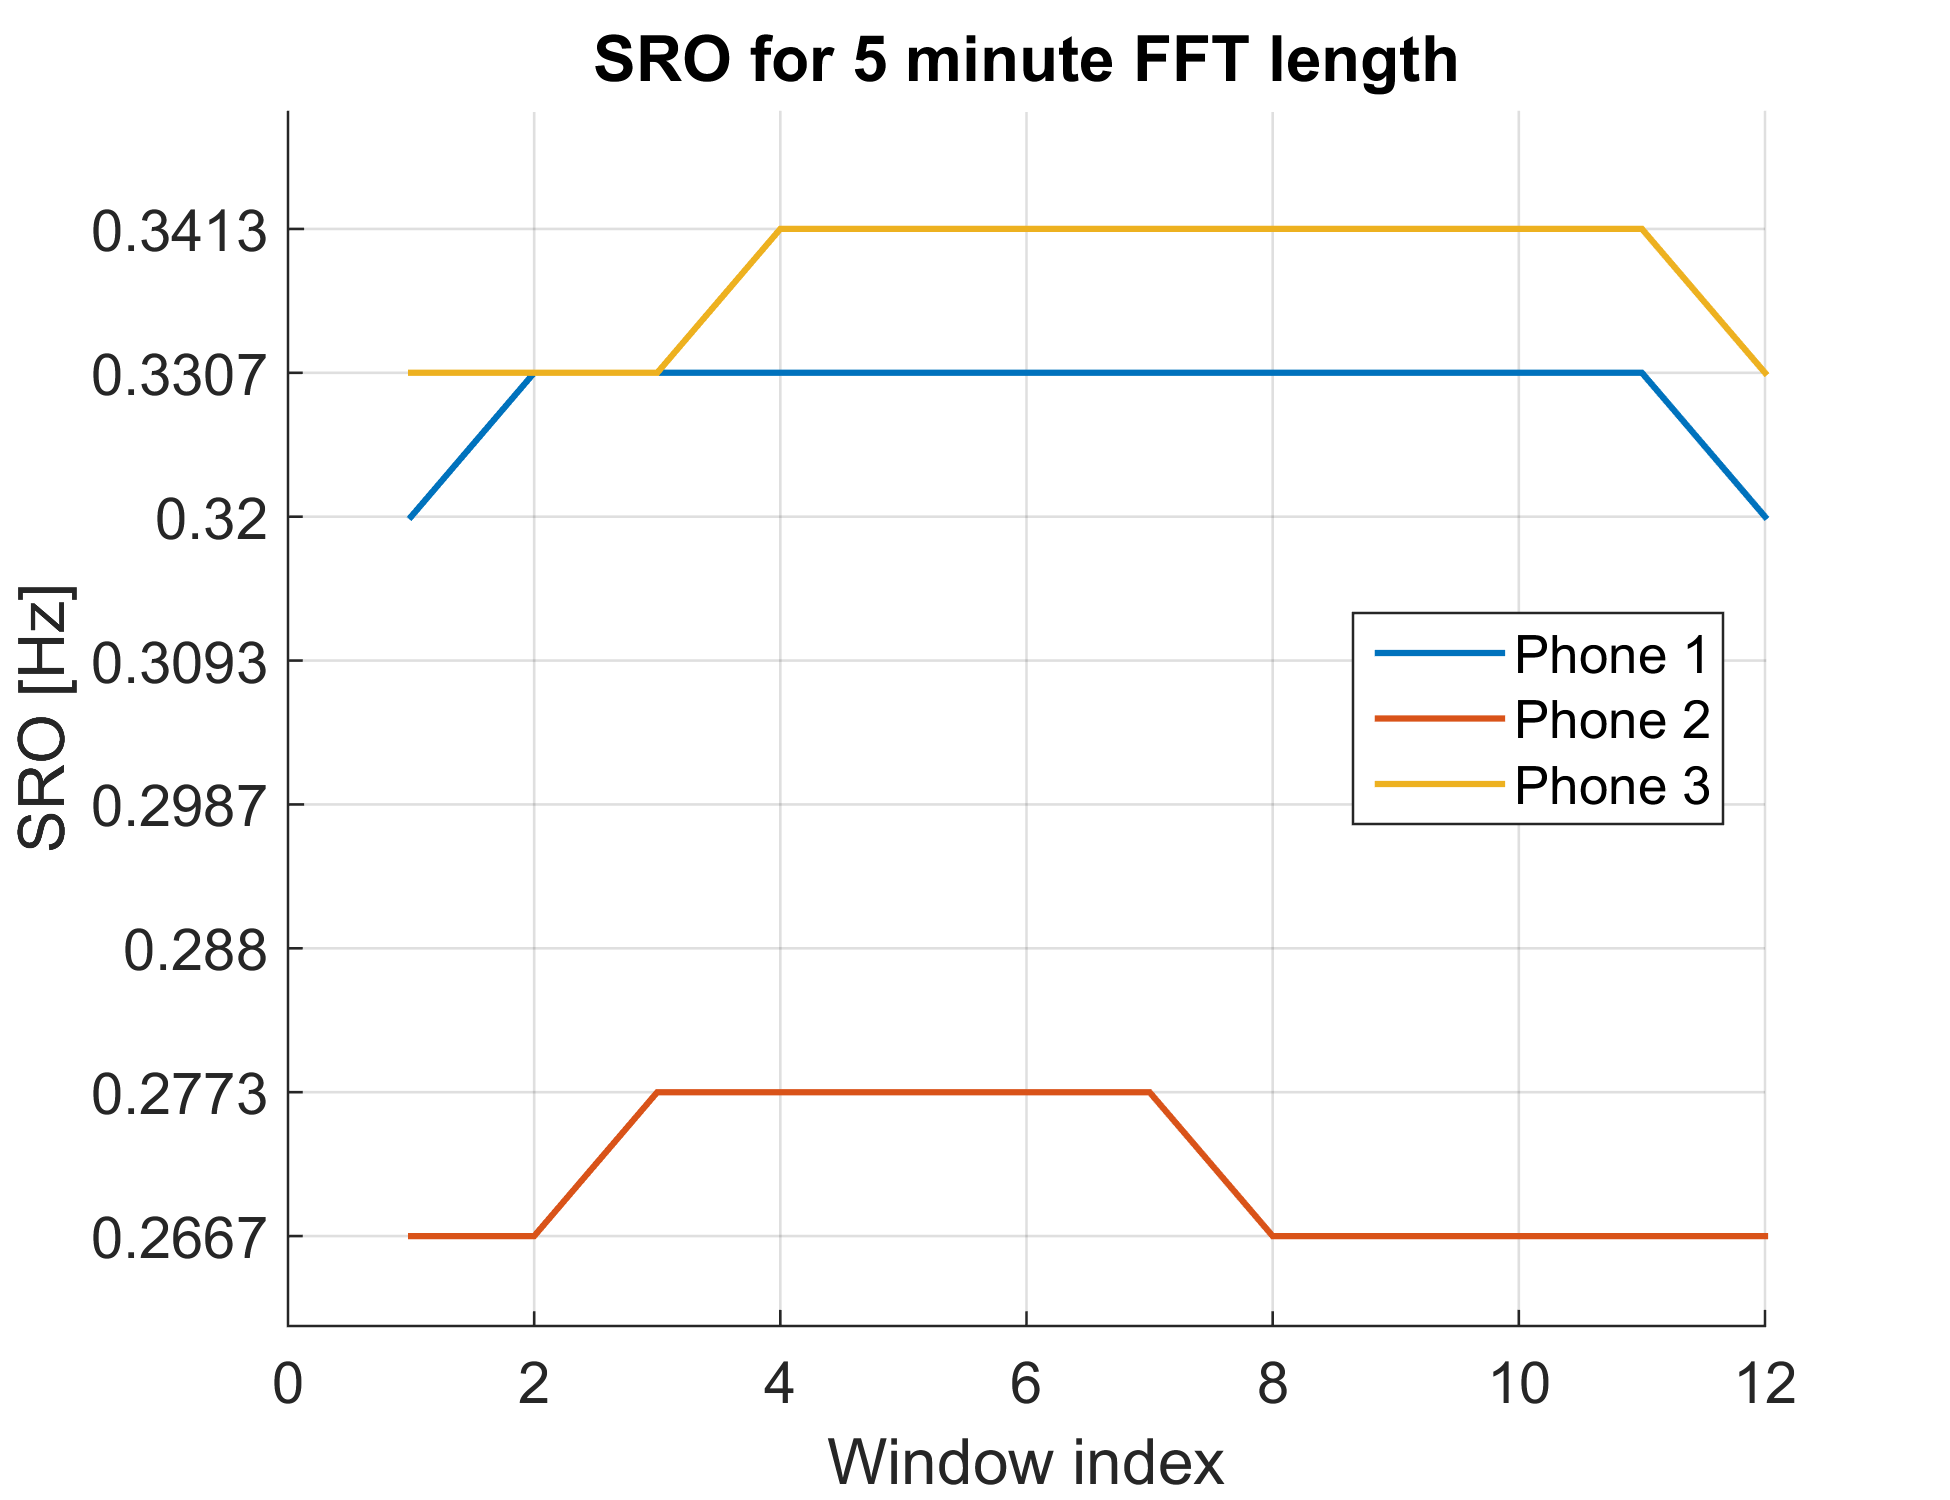
\includegraphics[width=\textwidth]{figures/sro-measurement/sro-5min}
		\caption{5 minute FFT window, $\Delta f=33~\mathrm{mHz}$.}
		\label{app:sro_5min}
	\end{subfigure}	
\end{adjustwidth}
\caption[Complete SRO measurement results.]{Sampling rate offset measurements for different FFT window lengths. A larger FFT window gives a higher frequency resolution $\Delta f$ but lower time resolution.}
\label{app:sro_total}
\end{figure}

\section{Real-life synchronization results}
\begin{figure}[H]
\begin{adjustwidth}{-1in}{-1in}
\centering
\begin{subfigure}{0.5\textwidth}
	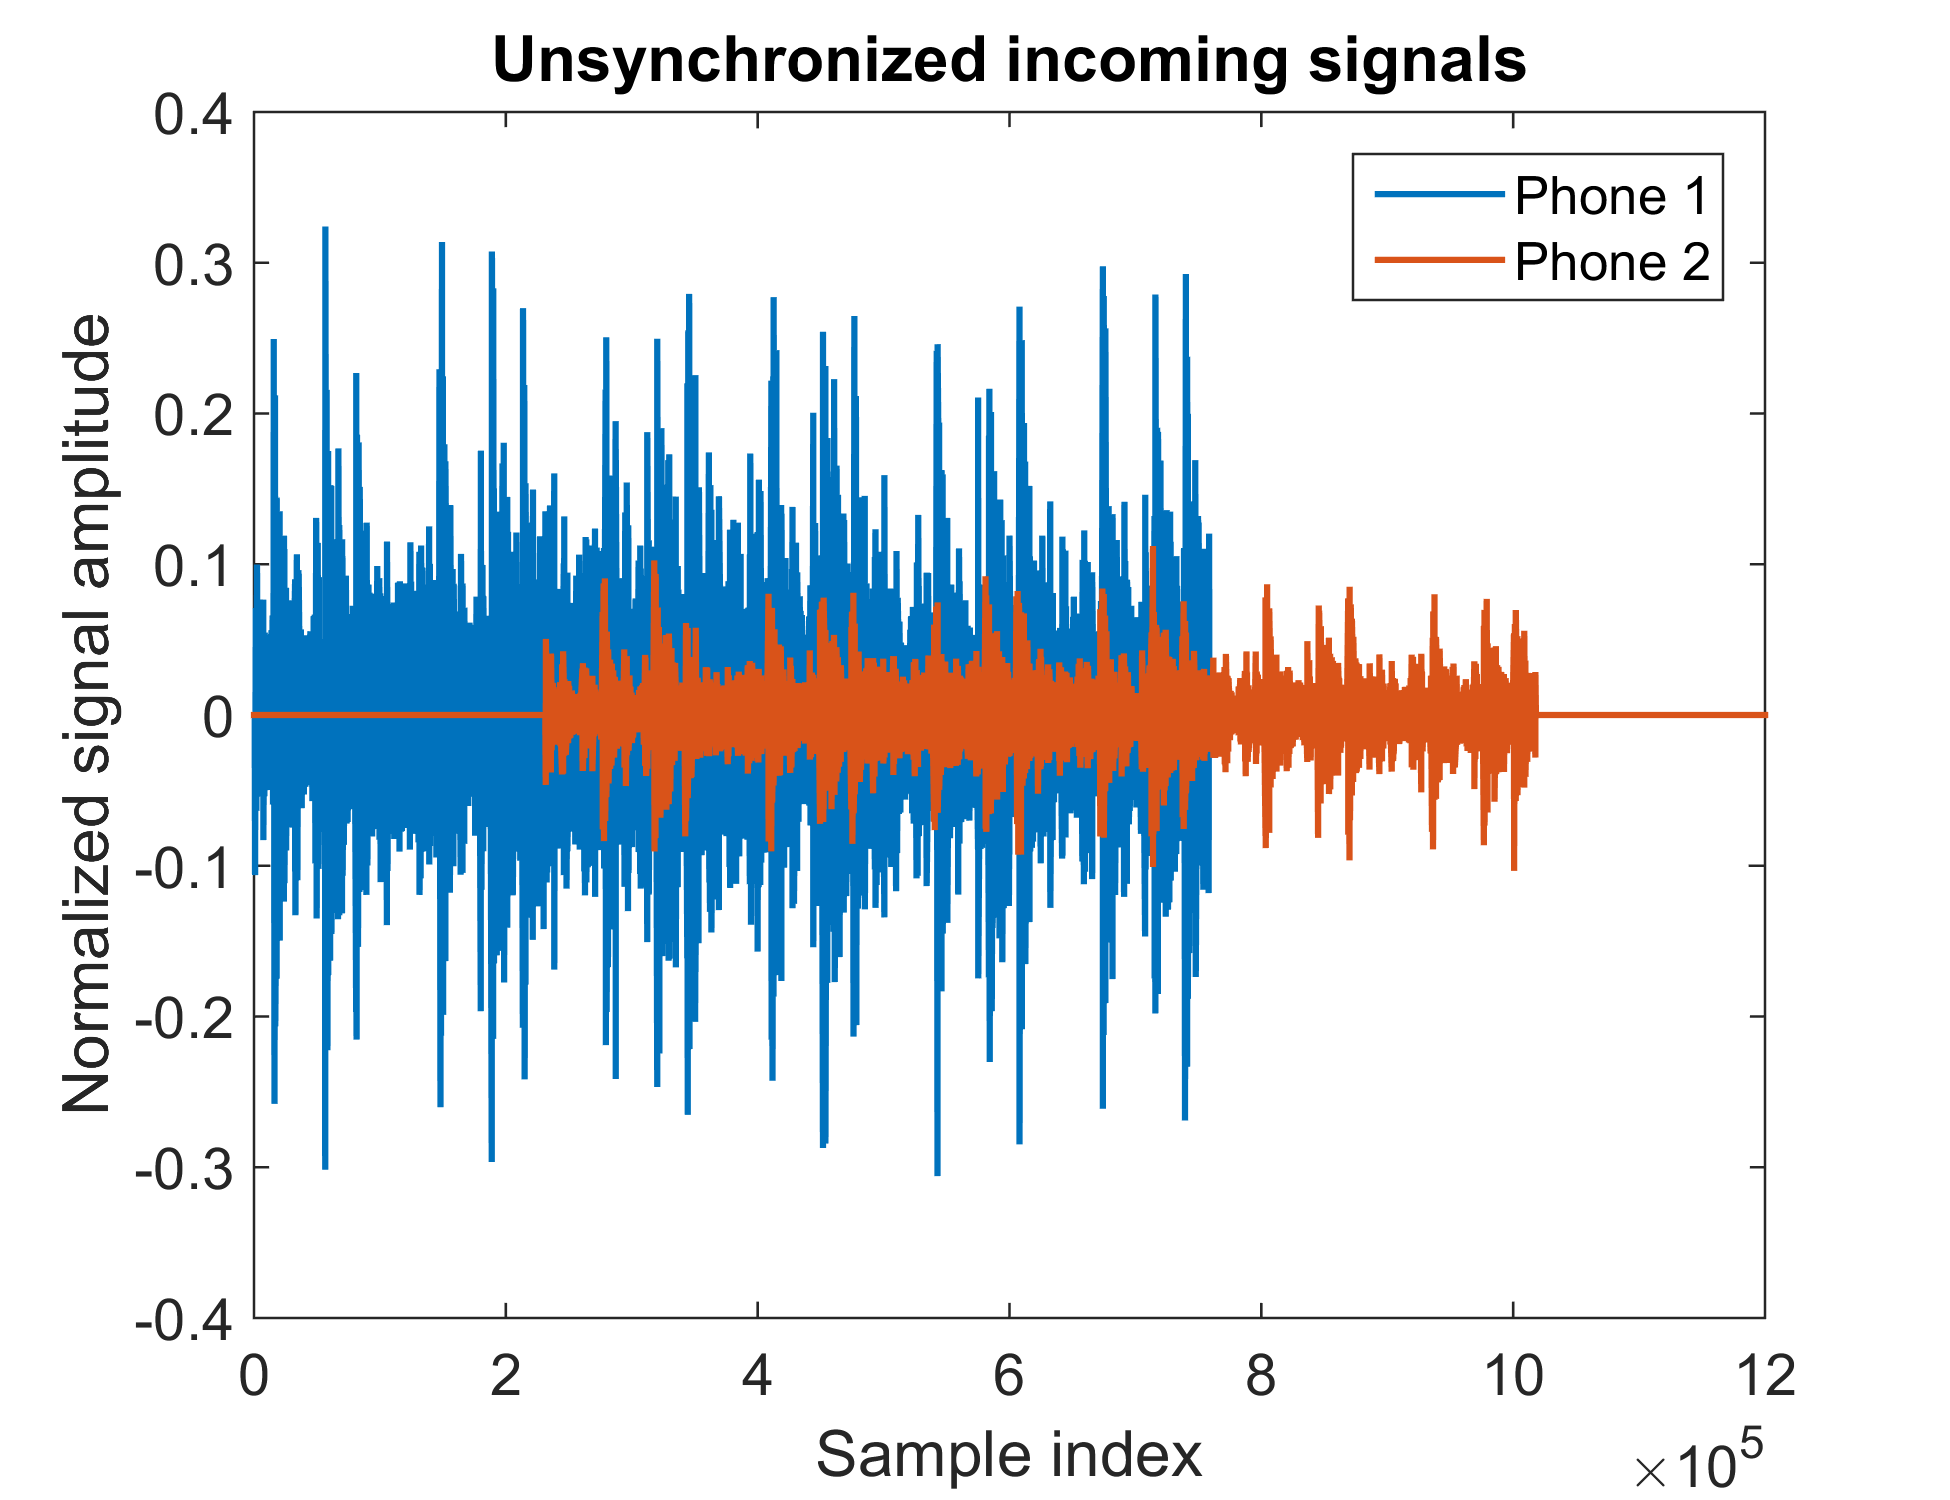
\includegraphics[width=\textwidth]{figures/system_test/result_unsynced}
	\caption{Unsynchronized smartphone audio.}
	\label{app:result_unsynced}
	\end{subfigure}
\begin{subfigure}{0.5\textwidth}
	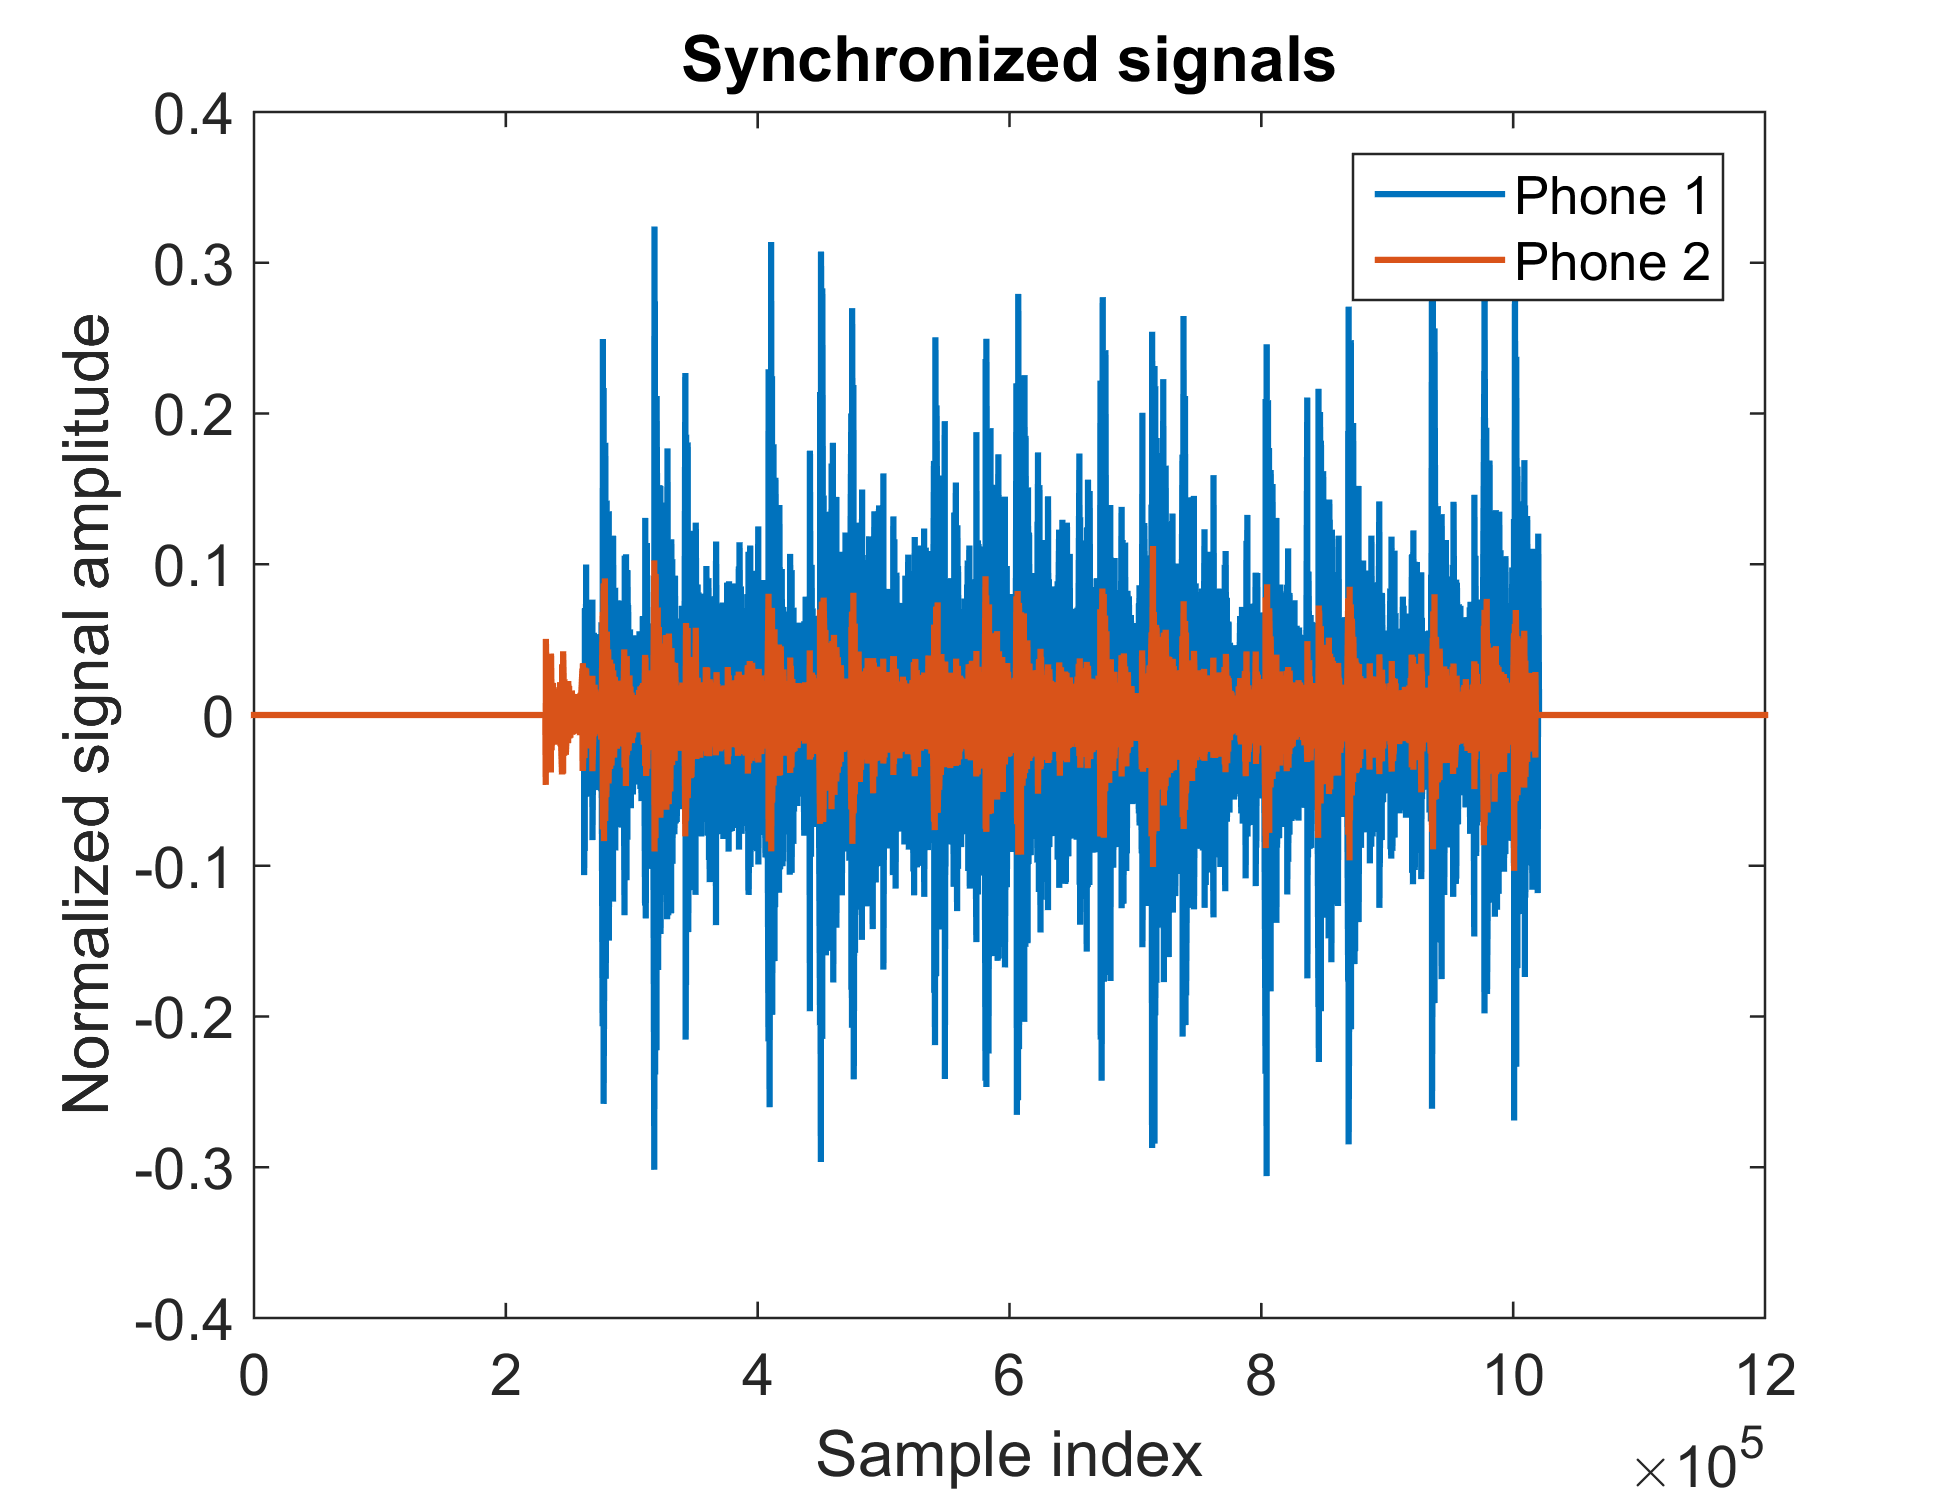
\includegraphics[width=\textwidth]{figures/system_test/result_synced}
	\caption{Synchronized smartphone audio.}
	\label{app:result_synced}
\end{subfigure}
\caption[Synchronization in a real-world scenario.]{Before (\ref{app:result_unsynced}) and after synchronization (\ref{app:result_synced}) of received audio in a real-life scenario. This is analogous to Figs. \ref{fig:sync-ex1}-\ref{fig:sync-ex2}. The recordings correspond to the ``Music (low MLS volume)'' measurement in table \ref{tab:test-result}.}
\label{app:result_synced_unsynced}
\end{adjustwidth}
\end{figure}

\chapter{Global coordinate system used by smartphone}

\begin{figure}[ht]
\centering
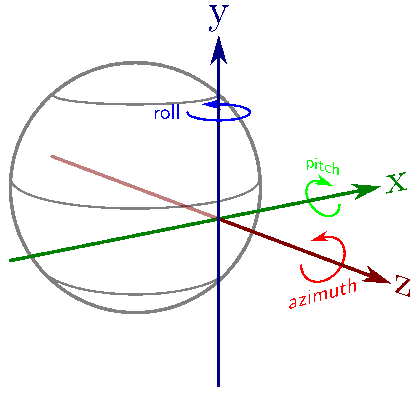
\includegraphics{figures/orientation/coordinate_system}
\caption[Global coordinate system for smartphones.]{The global coordinate system used for the smartphones in this work.}
\label{app:coordinate_system}
\end{figure}

\chapter{Ethical considerations}
This chapter in the thesis is not technically part of the thesis. It describes some ethical considerations related to (smartphone) microphone arrays and their applications. This chapter is included in all thesis works of the project group, e.g. also the work of Van Wijngaarden and Wouters \cite{BAP:ErikNiels} and Brinkman and De Rooij \cite{BAP:RosalieTim}. This chapter contains \emph{opinions} of the authors and is not a technical document.

\section*{The need for ethical discussion}
In creating the beamforming system, we envisioned a single purpose: speech enhancement in ad-hoc teleconference calls. Unfortunately, history teaches us some well-intended inventions turn out to be dangerous to the point where regulation is needed to ban it. Examples are numerous: tetraethyllead was added to gasoline starting in the 1920s but phased out worldwide from the 1970s because of its environmental impact. Radithor is another 1920s example; a ``wonder medicine'' in its heyday, it was subsequently discovered to be extremely toxic to the point that the main marketeer for the drugs' ``jaw fell off''.
Although these examples are very extreme, it is worthwhile examining the potential influence on society of our system-to-be.

\section*{Unintentional use cases}
The question we must ask ourselves thus becomes: what are some possible unforeseen use cases of our product? The possibility of a surveillance state (or company) using ad-hoc beamforming techniques to snoop on all its residents springs to mind. The revelations of NSA whistle blower Edward Snowden have documented just how far some American and European states are willing to go to keep tabs on their citizens. Moreover, they have revealed great levels of cooperation from tech-industrial giants such as Google, Facebook, Apple and others.

\section*{Beamformer contribution}
But how much would a smartphone beamforming system contribute to any level of mass-surveillance? The truth is that beamformers only work when the locations of smartphones are known to extreme accuracy. Such accuracy is not achievable with sensors fitted on even the latest smartphones. Furthermore, indoor localization of smartphones has thus far always relied on either large, extra hardware (RF beacons) or a sonic beacon. Neither seem appropriate to a state wanting to covertly listen in on conversations.

\section*{Applications}
Our prime focus has been with companies deploying the technology in teleconferencing situations. We do not seek out to be the next Skype, Hangouts or appear.in. A company using such software must be fully aware of the consequences of privacy invasion or potential information leakage caused by such software. Our solution would not be connected directly to the internet; it could, for example, serve as a virtual microphone input to the computer. What is done with the recorded audio is completely up to the user. 

\section*{Final remarks}
Theoretically, if the technology becomes more mature, it may become a weapon in the arsenal of surveillance states. But the technology is not remotely there yet. Ad-hoc beamforming on smartphones is still relatively uncharted territory and the lack of silent, unnoticable synchronization options kills off a potential to listen in discretely.
We honestly see no potential for abuse of the technology investigated in our research. 

\end{document}
